% !TeX root = ../main.tex
% 保留学校模板的三个栏目、研究计划表和末页备注栏。
% 3.1 为共同表征定义、时空结构理论及动作条件演化理论。
% 3.2 为总体技术路线及四项分项技术路线；3.3 为公开数据、分项验证及科学问题分析。
% 第二栏 3.4--3.6 为可行性、研究条件及问题应对；第三栏填写模板计划表及预期成果。
% 2026-10-30：以基础研究为定位；公开数据与标准学术评价支撑验证，机制示意不构成应用实验承诺。
% 第一个栏目及填写要求在主文件中给出。

\subsection{主要理论}

\subsubsection{三维场景表示与高斯泼溅}

三维场景表示旨在通过一定的数据结构或数学模型描述真实环境的空间几何与外观属性，是三维重建、场景理解及新视角合成的基础。常见的三维表示包括点云、三角网格、隐式神经场和显式几何图元等。点云通过离散空间采样描述物体形状，三角网格利用顶点与面片表达连续表面，隐式场通过连续函数表示空间密度或表面距离，显式图元则利用具有位置、尺度及外观属性的基本单元构建场景。不同表示形式在几何表达能力、存储开销及渲染效率方面具有不同特点。

三维高斯泼溅（3D Gaussian Splatting，3DGS）是一种基于显式高斯图元的三维场景表示与可微渲染方法\cite{gs2023}。该方法使用一组三维各向异性高斯描述场景，每个高斯图元包含中心位置、协方差、不透明度及颜色等属性。其中，三维高斯的空间分布可表示为

\begin{equation}
  G_i(\mathbf{x})=\exp\left(
-\frac{1}{2}(\mathbf{x}-\boldsymbol{\mu}_i)^\top
\boldsymbol{\Sigma}_i^{-1}
(\mathbf{x}-\boldsymbol{\mu}_i)
\right),
  \label{eq:route-gaussian-distribution}
\end{equation}
其中，$\mathbf{x}\in\mathbb{R}^3$ 为空间位置，$\boldsymbol{\mu}_i\in\mathbb{R}^3$ 为第 $i$ 个高斯的中心，$\boldsymbol{\Sigma}_i\in\mathbb{R}^{3\times3}$ 为其协方差矩阵。协方差通常通过旋转矩阵与尺度参数构造，以保证其对称正定性，并描述高斯图元在不同空间方向上的形状和范围。

在渲染过程中，三维高斯经过相机投影形成图像平面上的二维高斯分布，并根据深度顺序进行颜色与透明度合成。对于给定像素，其颜色可以表示为
\begin{equation}
  \mathbf{C}=\sum_{i=1}^{N}
  \mathbf{c}_i\alpha_i
  \prod_{j=1}^{i-1}(1-\alpha_j),
  \label{eq:route-gaussian-color}
\end{equation}

其中，$N$ 为参与该像素合成的高斯数量，$\mathbf{c}_i$ 为对应高斯的颜色，$\alpha_i$ 为由不透明度及投影高斯分布共同确定的像素贡献权重。通过可微渲染，可以利用图像重建误差对高斯图元的几何及外观参数进行优化。三维高斯表示兼具显式空间参数与高效渲染能力，为三维场景的可视化、重建及后续动态扩展提供了基础。


\subsubsection{动态场景表示与连续时间运动}

与静态场景不同，动态场景中的物体位置、几何形状及外观可能随时间发生变化，因此需要在三维空间表示中进一步引入时间维度。动态场景表示通常需要描述场景在不同时刻的状态及其相互联系。常见方式包括直接建立时变几何表示，以及通过运动或形变映射描述场景单元随时间的变化。后者通过建立参考状态与不同时刻之间的空间映射，使几何信息能够在时间维度上建立联系\cite{dnerf2021,nerfies2021,nsff2021,dynamicgs2024,gs4d2024}。

运动可以采用离散时间或连续时间形式进行描述。离散时间表示记录一系列采样时刻的空间位置与运动信息，连续时间表示则利用以时间为自变量的函数描述运动过程。对于参考位置为 $\mathbf{x}_0$ 的场景点，设其运动映射 $\Phi(\mathbf{x}_0,t)$ 关于时间 $t$ 可微，则该点在时刻 $t$ 的位置及瞬时速度可写为
\begin{equation}
  \mathbf{x}(t)=\Phi(\mathbf{x}_0,t),
  \qquad
  \mathbf{v}(t)=\frac{\partial\Phi(\mathbf{x}_0,t)}{\partial t},
  \label{eq:plan-motion-mapping}
\end{equation}
其中，$\Phi$ 表示随时间变化的空间映射，$\mathbf{v}(t)$ 为位置对时间的一阶导数。连续时间表示允许在函数定义域内查询非采样时刻的运动信息，常见参数化形式包括多项式、样条函数及神经网络等。其实际恢复精度仍取决于观测条件、函数表达能力及所采用的运动假设。

根据场景的运动性质，可以进一步区分刚体运动与非刚性形变。刚体运动保持物体内部任意两点之间的距离不变，通常由旋转和平移描述，其空间变换属于特殊欧氏群 $\mathrm{SE}(3)$。对于参考位置 $\mathbf{x}_0$，刚体运动可表示为
\[
  \mathbf{x}(t)=\mathbf{R}(t)\mathbf{x}_0+\mathbf{p}(t),
  \qquad
  \mathbf{R}(t)\in\mathrm{SO}(3),
\]
其中，$\mathbf{R}(t)$ 和 $\mathbf{p}(t)$ 分别表示旋转矩阵与平移向量。刚体变换满足任意两点之间的距离保持关系：
\[
  \|\mathbf{x}_i(t)-\mathbf{x}_j(t)\|_2
  =
  \|\mathbf{x}_{i,0}-\mathbf{x}_{j,0}\|_2.
\]
非刚性形变则允许物体内部的相对位置发生变化，需要更一般的空间映射进行描述。在实际动态场景中，不同区域可能具有不同的运动形式，局部运动也可能仅在特定时间区间内满足相应的连续性或刚性假设。




\subsubsection{空间结构与拓扑关系}

三维场景不仅包含几何元素及其运动信息，还具有由对象、部件及其相互关系构成的空间组织结构。从不同抽象层次出发，场景可以表示为基本几何单元的集合，也可以进一步组织为具有独立身份的对象及其内部部件。对象级表示侧重区分不同实体，部件级表示则描述对象内部具有一定几何或运动联系的组成部分。层次化空间组织能够在不同粒度上描述场景结构及其关系。

空间关系可以根据几何、运动或结构约束属性进行定义，例如空间邻近、包含、接触、共同运动、材料连续性及部件装配关系等。图结构是描述元素及其关系的一种常见数学形式，可表示为
\[
  \mathcal{H}=(\mathcal{V},\mathcal{E}),
  \qquad
  \mathcal{E}=\bigcup_{r\in\mathcal{R}}\mathcal{E}^{(r)},
\]
其中，$\mathcal{V}$ 为节点集合，$\mathcal{E}$ 为关系集合，$\mathcal{R}$ 表示关系类型集合，$\mathcal{E}^{(r)}$ 表示第 $r$ 类关系对应的边集合。节点可以对应空间点、几何单元、部件或对象，不同类型的边则用于描述几何邻近、运动关联或结构约束等关系。几何邻近、运动相似与结构约束属于不同性质的关系：空间相邻、接触或共同运动本身均不足以证明两个区域之间存在持续的结构约束。

拓扑结构主要描述空间对象的连通性等性质，以及这些性质在连续形变下的保持关系。切割、撕裂等过程可能破坏材料连续性并产生新的物理边界；部件装配关系则可以在不产生新表面的情况下改变或解除，例如旋合部件从受限连接转为分离。因而，结构约束关系的变化不必然等同于材料拓扑变化。关系图中的边变化也不自动表示真实结构改变：基于距离或运动相似性建立的关联可能随场景表征更新，而遮挡解除导致已有表面首次进入视野只是可见性变化。动态场景需要分别表示几何变化、观测可见性、材料连通性与部件间约束关系，并为关系及其运动约束记录类型和有效范围。



\subsubsection{状态空间模型与动态演化}

状态空间模型（State-Space Model）是描述动态系统内部状态及其演化规律的经典数学框架。该模型通常通过状态转移关系描述系统随时间的变化，并通过观测关系建立内部状态与外部测量之间的联系。在离散时间条件下，一般状态空间模型可以写为
\begin{equation}
\begin{aligned}
  \mathbf{s}_{k+1} &= F(\mathbf{s}_k,\mathbf{a}_k,\boldsymbol{\epsilon}_k),\\
  \mathbf{o}_k &= H(\mathbf{s}_k,\boldsymbol{\eta}_k),
\end{aligned}
\label{eq:plan-state-space}
\end{equation}
其中，$\mathbf{s}_k$ 为时刻 $k$ 的系统状态，$\mathbf{a}_k$ 为外部动作或控制输入，$\mathbf{o}_k$ 为观测结果，$\boldsymbol{\epsilon}_k$ 和 $\boldsymbol{\eta}_k$ 分别表示过程噪声与观测噪声。状态转移函数 $F$ 描述当前状态与动作共同决定的后续演化，观测函数 $H$ 描述系统状态产生可观测信息的过程。对于连续时间系统，也可以利用微分方程描述状态变化率及其与外部输入的关系。

在部分可观测条件下，系统的真实内部状态通常无法直接获取，需要根据已有观测与动作历史进行估计。部分可观测马尔可夫决策过程（Partially Observable Markov Decision Process，POMDP）为此提供了经典理论框架\cite{pomdp1998}。在状态满足马尔可夫假设时，贝叶斯滤波通过状态预测和观测更新两个步骤递推估计状态分布，其基本关系为
\begin{equation}
\begin{aligned}
  \bar b_{k+1}(\mathbf{s})
  &= \int p(\mathbf{s}\mid\mathbf{s}',\mathbf{a}_k)\,
  b_k(\mathbf{s}')\,d\mathbf{s}',\\
  b_{k+1}(\mathbf{s})
  &\propto p(\mathbf{o}_{k+1}\mid\mathbf{s})\,
  \bar b_{k+1}(\mathbf{s}),
\end{aligned}
\label{eq:plan-bayes-filter}
\end{equation}
其中，$b_k$ 表示根据已有信息形成的状态信念分布，$\bar b_{k+1}$ 表示动作条件下的预测分布，$b_{k+1}$ 表示结合新观测更新后的状态分布。上述过程体现了动态系统中状态演化与观测修正的基本关系。

世界模型将状态表示与环境演化预测相结合，通过学习状态转移规律，对给定条件下的未来状态或观测进行预测。学习式世界模型可以在显式物理状态、视觉特征或潜在状态空间中建立动态关系，并根据任务需要支持环境预测、过程推演及决策\cite{worldmodels2018,ref01,dreamer2020,ref02}。不同模型的状态表达形式与预测目标可能不同，但均涉及如何利用已有信息描述当前环境，以及如何根据状态和外部条件刻画后续变化的基本问题。


\subsection{研究方法}

本课题拟采用理论分析、算法设计与实验验证相结合的研究方法。首先，围绕有限视觉观测下动态表征的可区分性及动作响应预测所需的表征信息，分析连续运动、空间结构与动态演化的基本关系，明确相关问题的建模条件与研究边界；其次，结合计算机视觉、三维重建及机器学习等技术，开展连续时间场景表征、对象时空一致性建模、结构约束关系变化下的表征维护和动作后果预测等方面的算法研究；最后，依托公开数据集，通过基线对比、机制消融及误差分析，验证所提出方法的有效性，研究关键因素的作用及方法的适用条件。



\subsection{技术路线}
\label{sec:plan-route}

本课题围绕连续动态世界模型的构建，以有限时序视觉观测及可用几何先验为基础，通过连续时间运动恢复、对象时空一致性建模和结构约束关系变化下的表征维护，协同构建可持续更新的连续动态世界表征。在此基础上，结合交互历史学习响应相关潜在表征，以动作条件演化预测为目标进一步完善世界表征，形成表征构建、演化预测与观测修正相联系的模型框架。总体技术路线如图~\ref{fig:technical-route-overview} 所示。

\begin{figure}[H]
  \centering
  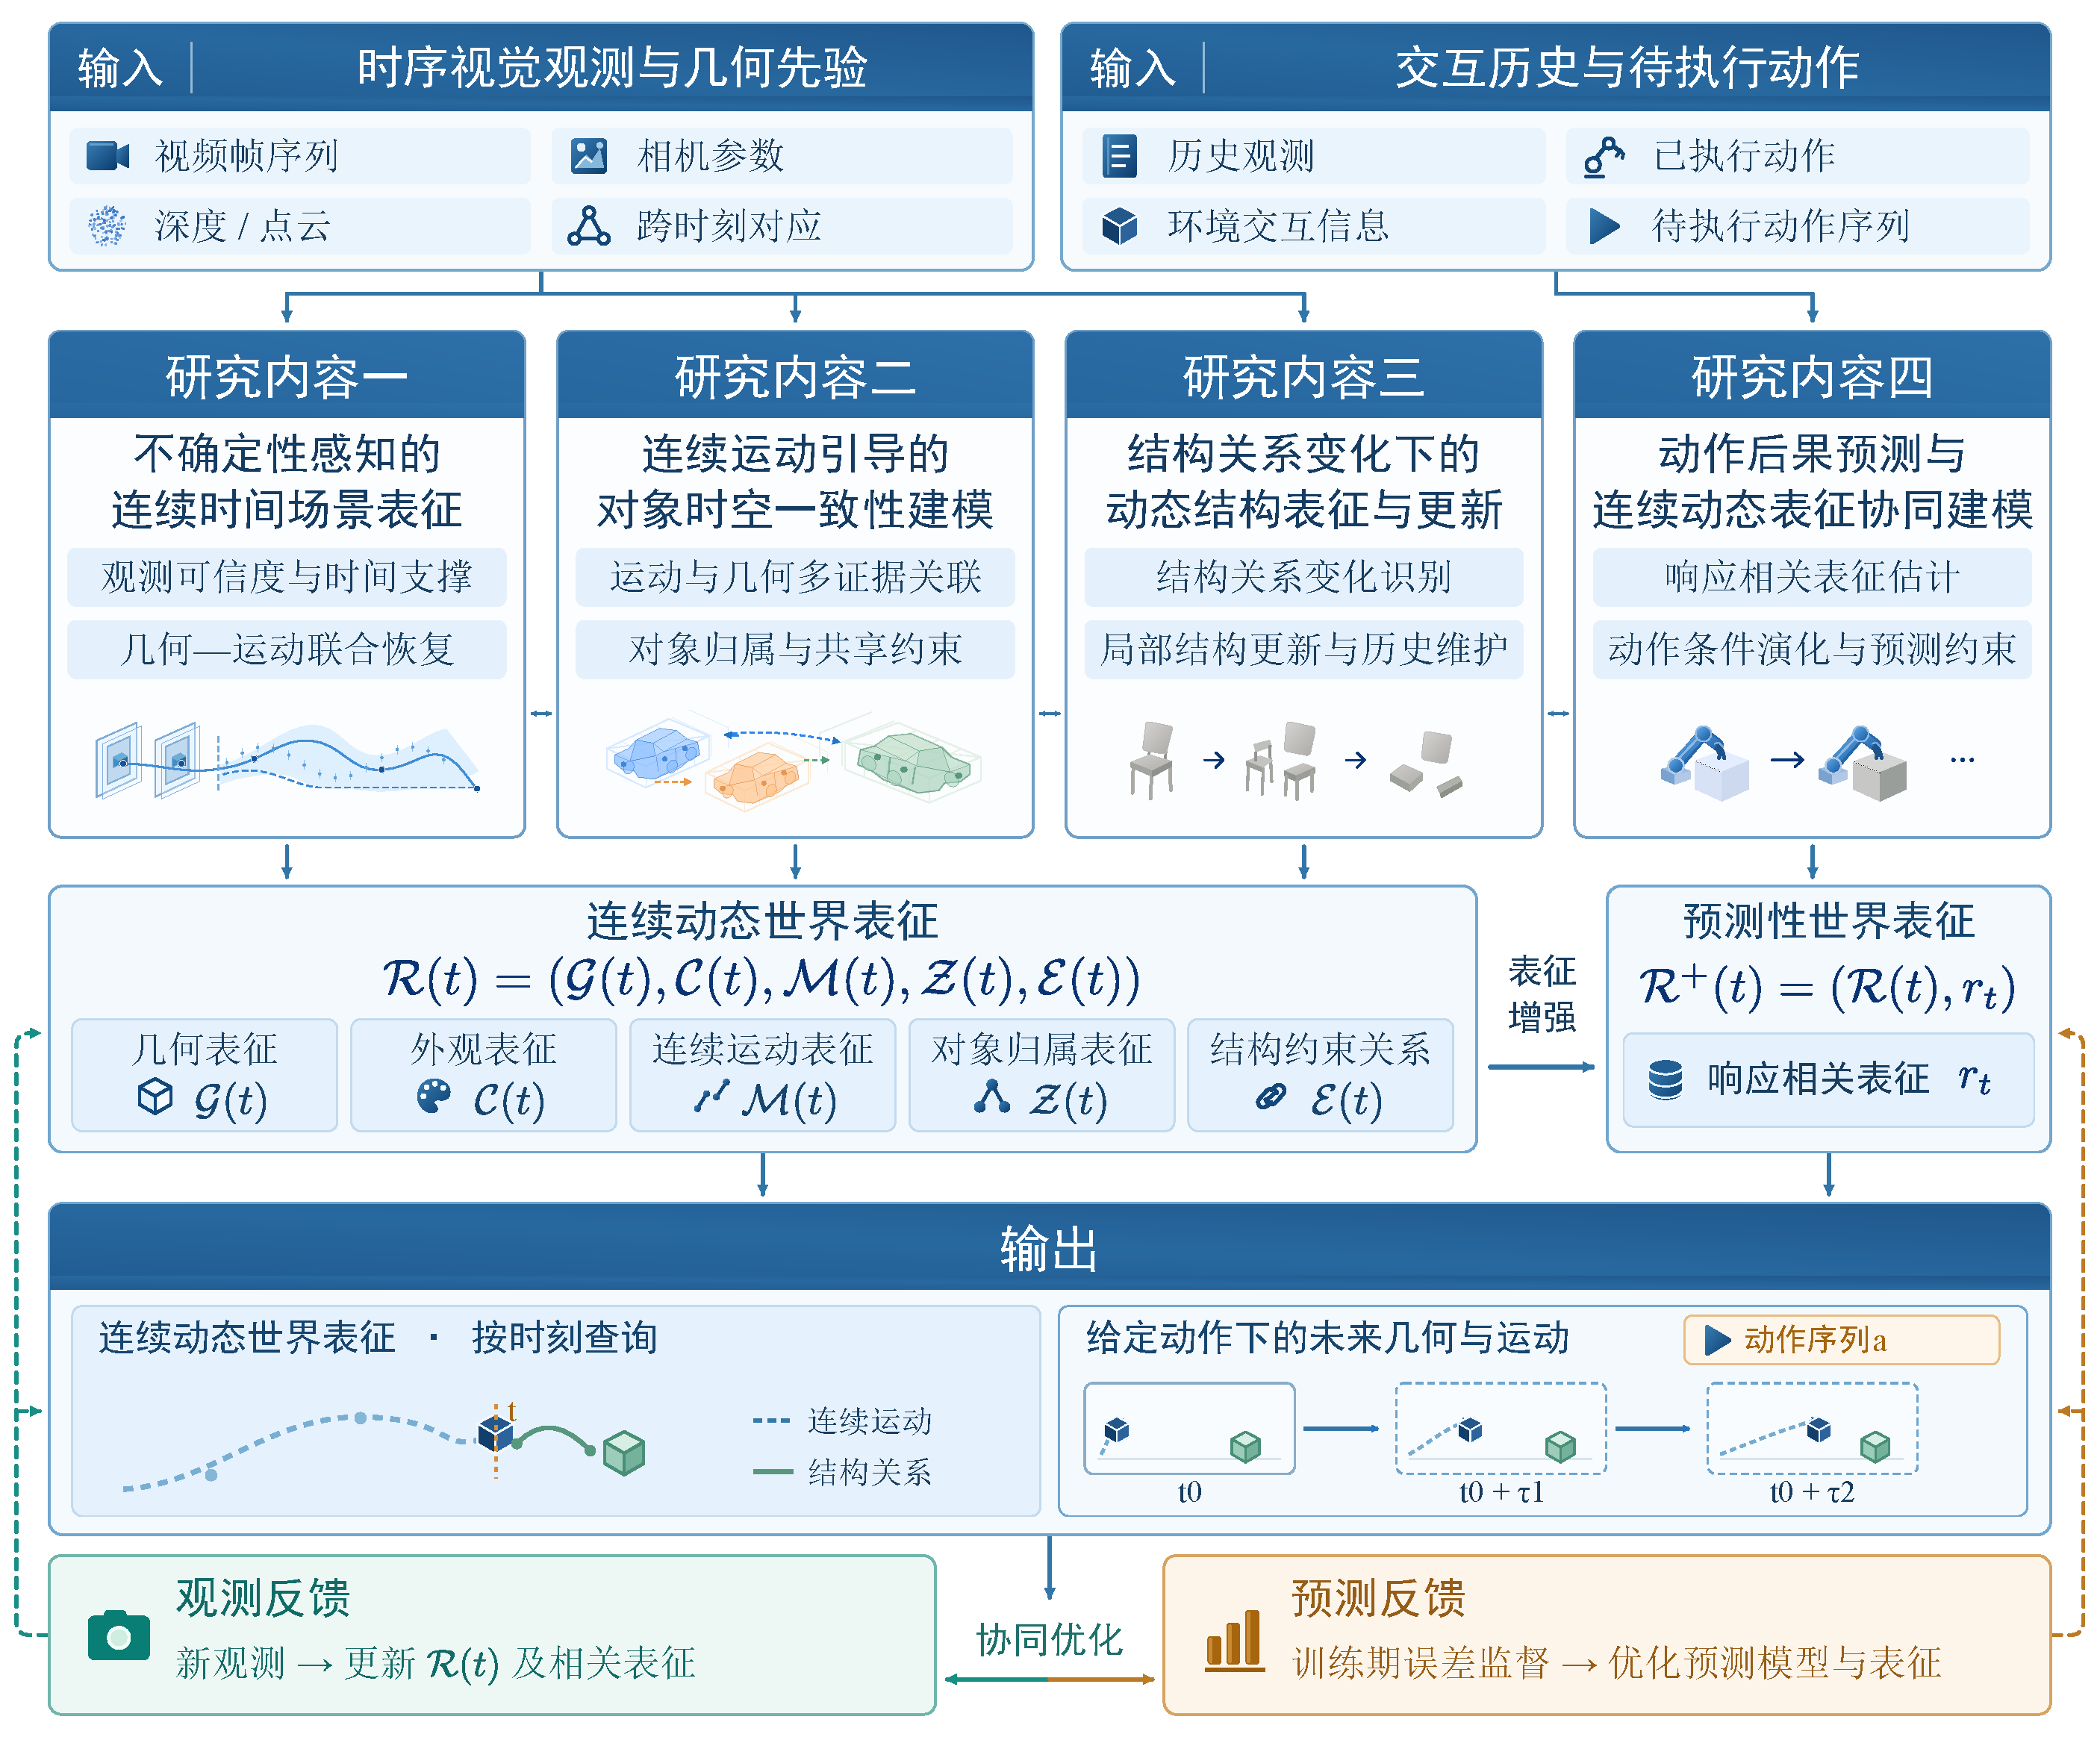
\includegraphics[width=\linewidth]{figures/chapters/ch03-plan/overall-technical-route/figure.pdf}
  \caption{连续动态场景表征与动作条件预测技术路线}
  \label{fig:technical-route-overview}
\end{figure}

为统一描述动态场景的几何、外观、运动及结构关系，本课题构建可按时间查询、可随观测更新的动态场景表征：
\begin{equation}
  \mathcal{R}(t)=
  \bigl(
    \mathcal{G}(t),
    \mathcal{C}(t),
    \mathcal{M}(t),
    \mathcal{Z}(t),
    \mathcal{E}(t)
  \bigr),
  \label{eq:plan-scene-representation}
\end{equation}
其中，$\mathcal{G}(t)$ 和 $\mathcal{C}(t)$ 分别表示场景的三维几何与外观表征，$\mathcal{M}(t)$ 表示连续运动表征，$\mathcal{Z}(t)$ 表示对象或部件的空间归属，$\mathcal{E}(t)$ 表示结构关系及其类型、运动约束支持与有效范围，涵盖部件装配约束和材料连续性等信息。连续动态场景表征可按时间查询，结构关系及其约束范围可依据新观测更新；材料断裂及新生表面通过其中相应的拓扑与表面信息表示。前三项研究围绕上述分量的连续恢复、空间组织与关系更新展开，协同构建时空一致的动态场景表征。

在此基础上，第四项研究结合截至预测起点 $t_0$ 的观测与交互历史，编码响应相关的潜在表征 $r_{t_0}$，将基础动态表征增强为预测性世界表征：
\begin{equation}
  \mathcal{R}^{+}(t_0)=
  \bigl(\mathcal{R}(t_0),r_{t_0}\bigr),
  \label{eq:plan-predictive-representation}
\end{equation}
并在给定动作条件下预测未来几何与运动响应，研究对象归属及当前结构约束关系对响应传播的影响，利用预测任务进一步约束和优化内部表征。四项研究的具体技术路线分别如下。






\subsubsection{不确定性感知的连续时间场景表征}
\label{sec:plan-time}

本项研究面向有限离散视觉观测下的连续运动与动态几何恢复，采用“可靠观测证据构建—观测驱动的连续运动建模—几何与运动联合恢复”的技术路线，如图~\ref{fig:plan-route-time} 所示。首先融合视觉基础模型提供的几何与跨时刻对应先验，构建具有可靠性和时间覆盖信息的观测约束；随后以稀疏运动支撑建立连续时间变形模型，根据观测支持自适应调整局部运动表达能力；最后结合三维高斯表示与多时刻联合优化，持续校正动态场景的几何和运动，并维护弱观测区域的运动不确定性。

\begin{figure}[H]
  \centering
  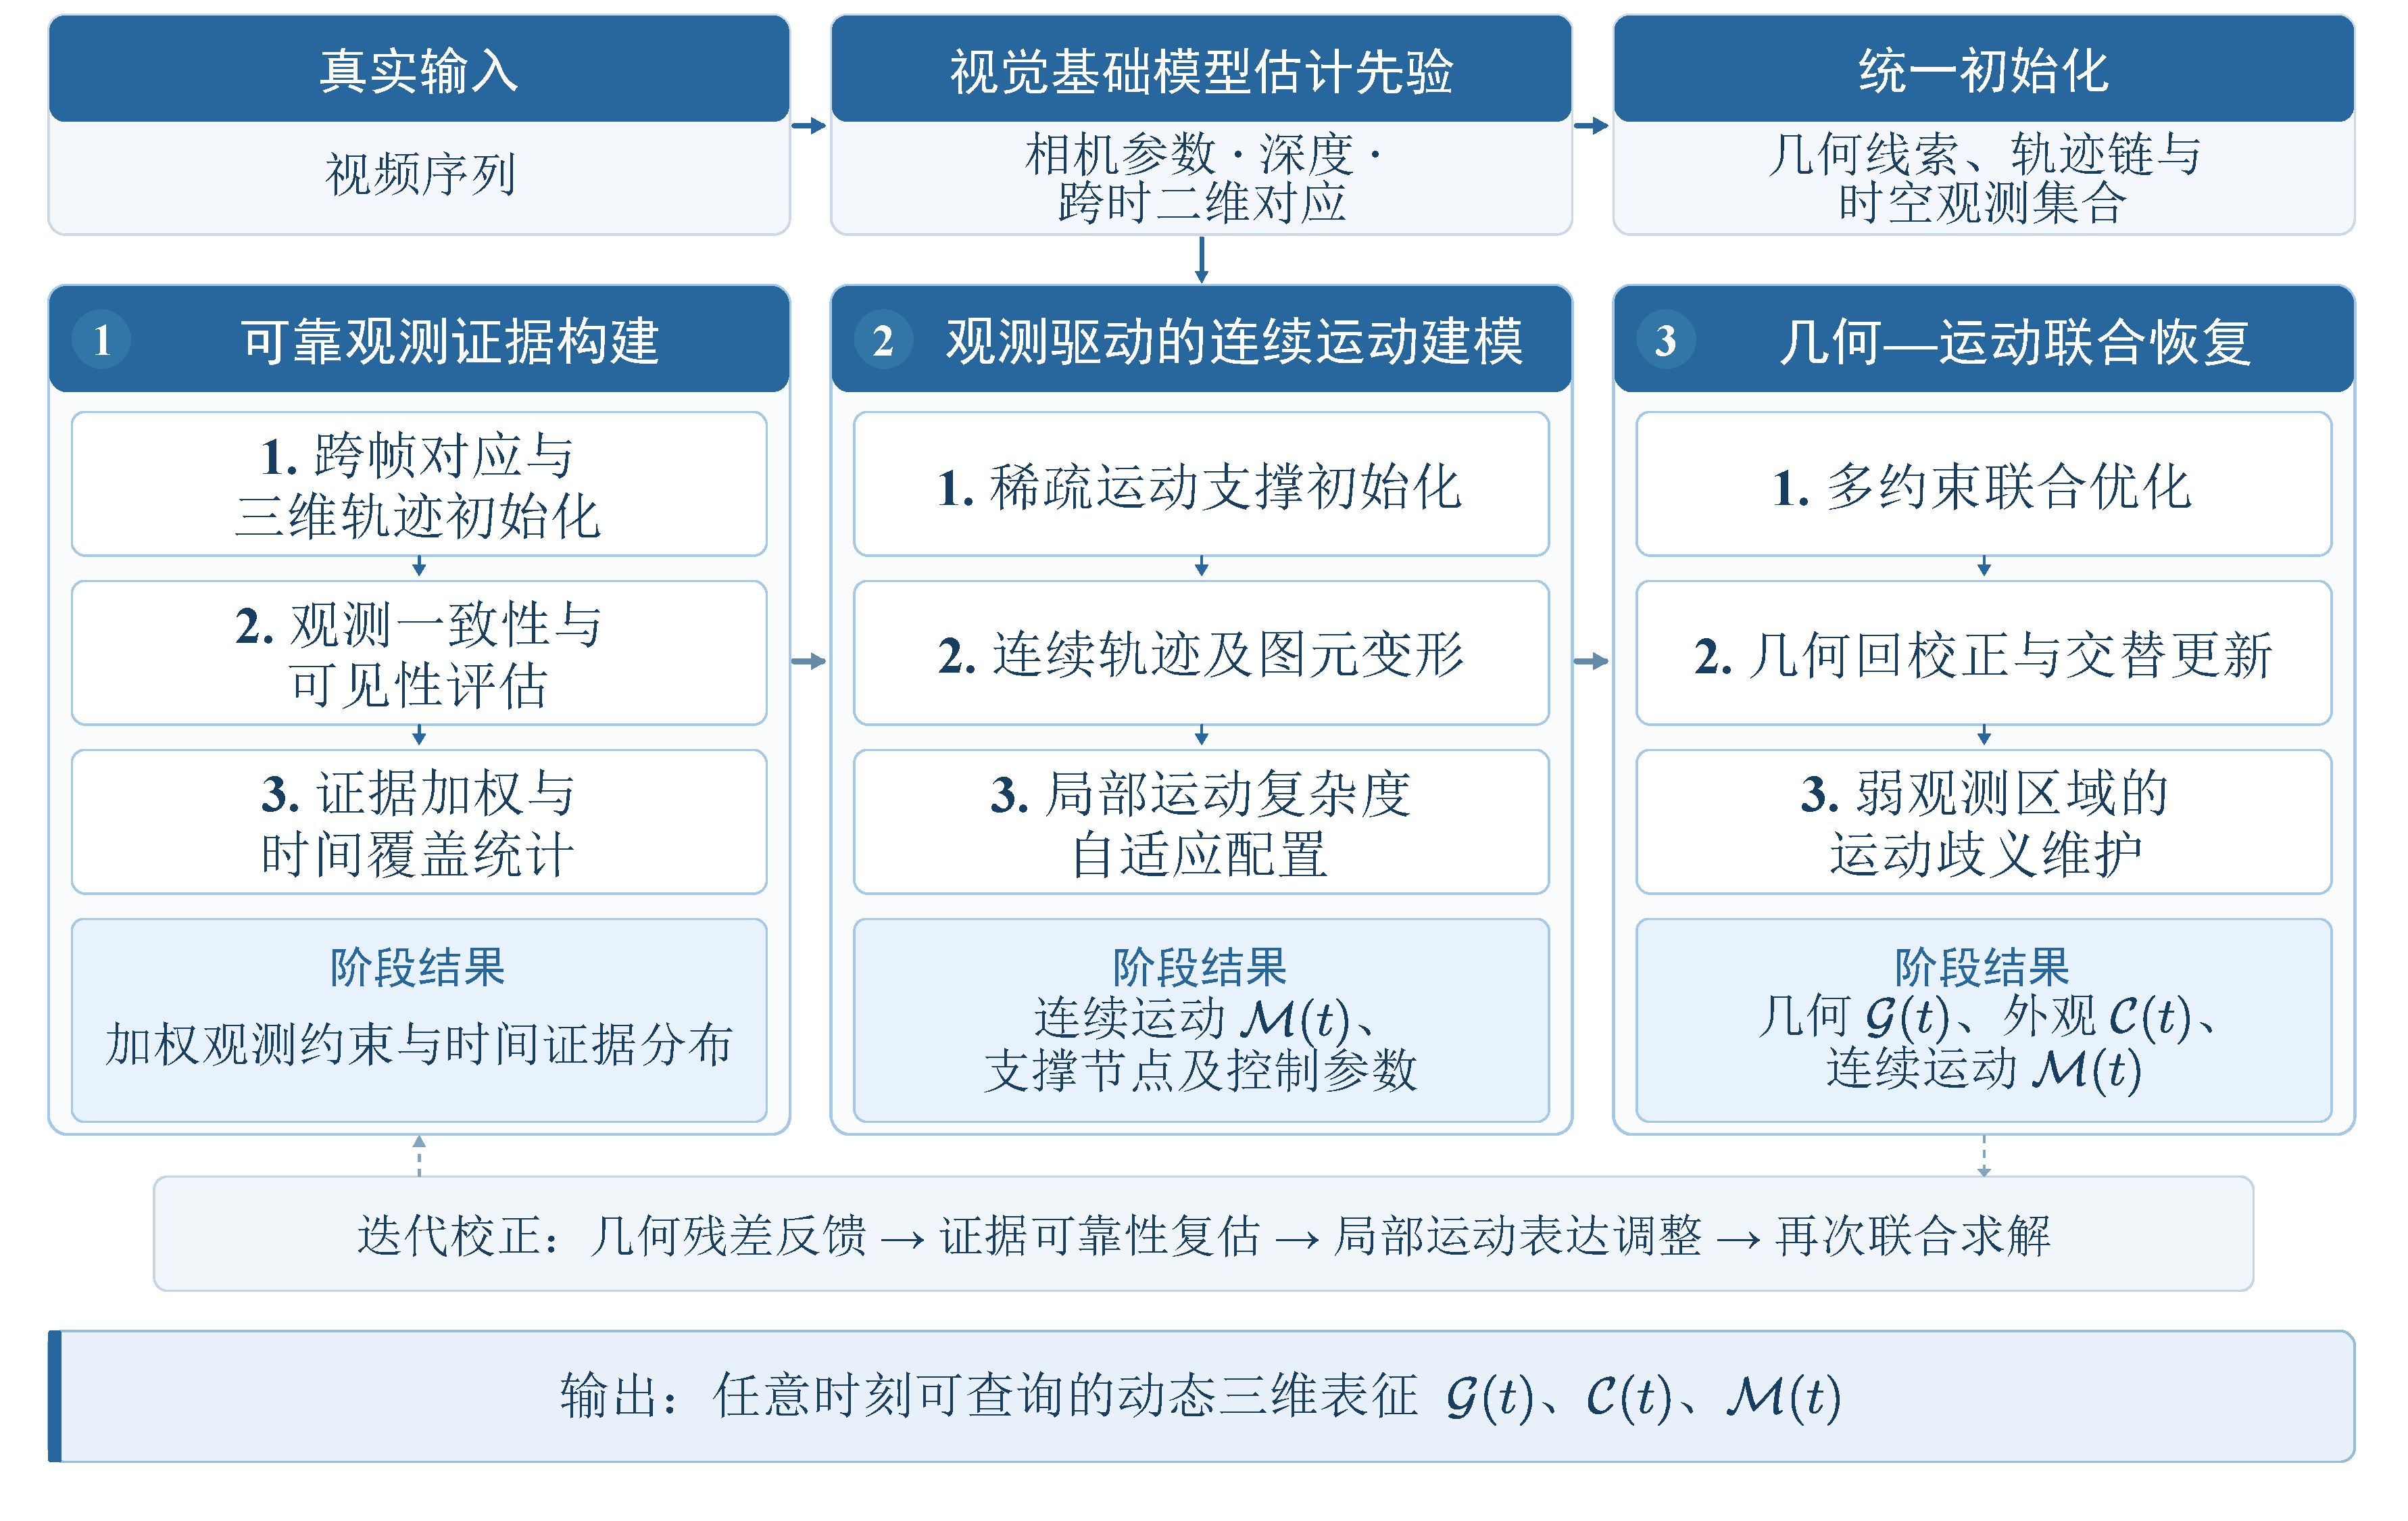
\includegraphics[width=\linewidth]{figures/chapters/ch03-plan/continuous-time-route/figure.pdf}
  \caption{不确定性感知的连续时间场景表征技术路线}
  \label{fig:plan-route-time}
\end{figure}

\noindent\textbf{（1）可靠观测证据构建}

设输入视频序列为 $\mathcal{I}=\{I_k\}_{k=1}^{N}$，对应采样时刻为 $\{t_k\}_{k=1}^{N}$。利用视觉基础模型获取相机参数、深度图及跨时刻二维对应，并通过深度反投影与坐标统一获得初始三维轨迹。对于轨迹 $a$ 在时刻 $t_k$ 的观测，综合对应一致性、几何一致性及可见性，构建可靠性权重 $w_{a,k}=c_{a,k}^{\mathrm{track}}c_{a,k}^{\mathrm{geo}}v_{a,k}$，以调节不同观测在后续运动恢复中的作用。

考虑动态场景各区域的时间采样和有效观测覆盖不同，进一步根据初步轨迹及候选运动支撑区域统计局部时间证据：
\begin{equation}
  H_j(t)=
  \sum_{a,k}
  \beta_{a,j}w_{a,k}\kappa_h(t-t_k),
  \label{eq:route-motion-temporal-support}
\end{equation}
其中，$\beta_{a,j}$ 为轨迹 $a$ 对候选支撑区域 $j$ 的关联权重，$\kappa_h$ 为局部时间核函数，$H_j(t)$ 表示该区域在时刻 $t$ 附近的有效观测支持。通过联合考虑观测可靠性和时间覆盖，建立加权时空约束，为后续连续运动建模提供可靠证据及局部约束强度依据。

\noindent\textbf{（2）观测驱动的连续运动建模}

根据三维轨迹的空间分布和运动一致性初始化稀疏运动支撑节点，以少量连续轨迹描述局部场景运动。设节点 $j$ 的参考位置为 $\mathbf{p}_j^0$，参考时刻为 $t_{\mathrm{ref}}$，采用样条基函数建立连续时间位置轨迹：
\begin{equation}
  \mathbf{p}_j(t)=
  \mathbf{p}_j^0+
  \sum_{\ell=1}^{L_j}
  \bigl[
    B_{j,\ell}(t)-B_{j,\ell}(t_{\mathrm{ref}})
  \bigr]\mathbf{c}_{j,\ell},
  \label{eq:route-motion-spline}
\end{equation}
其中，$B_{j,\ell}(t)$ 为时间基函数，$\mathbf{c}_{j,\ell}$ 为控制参数，$L_j$ 为局部时间控制参数数量。节点旋转 $\mathbf{R}_j(t)\in\mathrm{SO}(3)$ 采用连续旋转参数化描述，并满足参考时刻的旋转为单位矩阵。

对于参考时刻的三维位置 $\mathbf{x}$，由邻近运动节点的局部变换构建连续变形映射：
\begin{equation}
  \Phi(\mathbf{x},t)=
  \sum_{j\in\mathcal{N}(\mathbf{x})}
  \alpha_j(\mathbf{x})
  \left[
    \mathbf{R}_j(t)
    (\mathbf{x}-\mathbf{p}_j^0)
    +\mathbf{p}_j(t)
  \right],
  \label{eq:route-motion-deformation}
\end{equation}
其中，$\mathcal{N}(\mathbf{x})$ 为局部运动支撑集合，$\alpha_j(\mathbf{x})$ 为归一化的非负关联权重。该映射将稀疏运动轨迹传播至三维高斯图元，实现稠密动态几何的连续时间表达。

针对不同区域运动复杂度和观测支持的差异，拟结合时间覆盖与运动拟合残差，自适应调整局部样条控制点数量，并构建观测支持驱动的运动正则约束：
\begin{equation}
  \begin{aligned}
  \mathcal{L}_{\mathrm{motion}}
  &=
  \sum_j\int_{\mathcal{T}}
  \lambda_j(t)
  \left\|
    \frac{\partial^2\mathbf{p}_j(t)}
         {\partial t^2}
  \right\|_2^2\,\mathrm{d}t,\\
  \lambda_j(t)
  &=
  \lambda_{\min}
  +\frac{\lambda_0}{H_j(t)+\epsilon},
  \end{aligned}
  \label{eq:route-motion-adaptive-regularization}
\end{equation}
其中，$\lambda_j(t)$ 为局部运动平滑权重，$\mathcal{T}$ 为建模时间范围，$\lambda_{\min}$、$\lambda_0$ 为调节参数。控制点增减依据局部残差与时间支持共同判定：观测覆盖充分且残差持续偏大时增加表达自由度，证据有限时保持较低自由度；并在未参与拟合的采样时刻检查插值稳定性，若留出误差未改善则不再增加自由度，以避免过拟合观测噪声。节点瞬时速度由连续样条轨迹求导获得，避免依赖离散帧差分，并为后续动作预测提供一致的运动输入。通过运动表达复杂度与平滑强度的协同调整，使观测充分的区域能够刻画复杂运动变化，同时提高稀疏观测区域的轨迹估计稳定性。

\noindent\textbf{（3）几何—运动联合恢复}

在连续运动模型的基础上，采用三维高斯表示动态场景的几何与外观，通过连续变形更新图元属性，并利用可微渲染建立跨时刻观测约束。设几何、外观和运动参数分别为 $\Theta_G$、$\Theta_C$ 和 $\Theta_M$，构建联合优化目标：
\begin{equation}
  \min_{\Theta_G,\Theta_C,\Theta_M}\quad
  \mathcal{L}
  = \lambda_{\mathrm{trk}}\mathcal{L}_{\mathrm{trk}}
  + \lambda_{\mathrm{rgb}}\mathcal{L}_{\mathrm{rgb}}
  + \lambda_{\mathrm{dep}}\mathcal{L}_{\mathrm{dep}}
  + \lambda_{\mathrm{mot}}\mathcal{L}_{\mathrm{motion}}
  + \lambda_{\mathrm{reg}}\mathcal{L}_{\mathrm{reg}},
  \label{eq:route-motion-joint-objective}
\end{equation}
其中，$\mathcal{L}_{\mathrm{trk}}$ 为观测可靠性加权的轨迹重投影损失，$\mathcal{L}_{\mathrm{rgb}}$ 和 $\mathcal{L}_{\mathrm{dep}}$ 分别为图像重建与深度一致性损失，$\mathcal{L}_{\mathrm{motion}}$ 和 $\mathcal{L}_{\mathrm{reg}}$ 分别约束连续运动及局部几何变形。通过轨迹、渲染和几何信息的联合约束，使连续运动估计与三维高斯重建相互校正。

优化采用交替更新策略：首先利用重投影及渲染残差评估当前几何与运动估计，更新观测可靠性；随后根据局部时间支持和运动误差调整轨迹表达复杂度及正则强度；最后联合更新连续运动参数与三维高斯几何，逐步改善跨时刻一致性和非采样时刻的恢复精度。

针对遮挡及时间采样不足的区域，进一步通过不同观测子集或初始化获得多组候选轨迹，并根据其估计分歧描述局部运动不确定性：
\begin{equation}
  U_j(t)=
  \frac{1}{S}\sum_{s=1}^{S}
  \left\|
    \mathbf{p}_j^{(s)}(t)
    -\bar{\mathbf{p}}_j(t)
  \right\|_2^2,
  \label{eq:route-motion-uncertainty}
\end{equation}
其中，$\mathbf{p}_j^{(s)}(t)$ 为第 $s$ 组候选轨迹，$\bar{\mathbf{p}}_j(t)$ 为其均值，$S$ 为候选数量。结合有效观测支持 $H_j(t)$ 与运动分歧 $U_j(t)$，评估弱观测区域的运动估计稳定性，并指导局部运动约束与几何更新。随着新增观测到来，持续修正观测权重、连续运动及三维几何。

最终形成由几何 $\mathcal{G}(t)$、外观 $\mathcal{C}(t)$ 和连续运动 $\mathcal{M}(t)$ 构成的动态场景表征，支持在建模时间范围内查询连续运动与几何信息。拟通过不同时间采样密度、遮挡程度和运动复杂度下的受控实验，结合运动轨迹精度、非采样时刻重建质量及关键机制消融，验证观测可靠性建模、自适应运动表达和几何—运动联合优化的作用。




\subsubsection{连续运动引导的对象时空一致性建模}
\label{sec:plan-space}

本项研究面向遮挡、短时共动及局部形变条件下的对象时空一致性建模，采用“多证据空间关联—部件软归属与身份维护—归属约束的联合恢复”的技术路线，如图~\ref{fig:plan-route-object} 所示。首先利用连续运动、几何、外观与可见性建立具有可靠性评估的空间关联；随后通过部件身份锚点与软归属维护跨时刻空间组织，并根据观测证据更新待定关系；最后结合身份兼容和运动兼容约束局部信息共享，通过几何、运动与空间归属的联合优化，形成具有持续对象身份和时空一致性的动态场景表征。

本项区分空间关联、对象或部件身份与结构约束：邻近和短时共动只生成关联候选，分割先验不直接决定身份；结构约束单独描述关系支持的信息共享范围。观测不足或证据冲突时保留待定归属，再由新增观测更新。验证覆盖短时共动、部件相对运动、遮挡重现与首次显露，检查归属及共享范围能否随证据调整。

\begin{figure}[H]
  \centering
  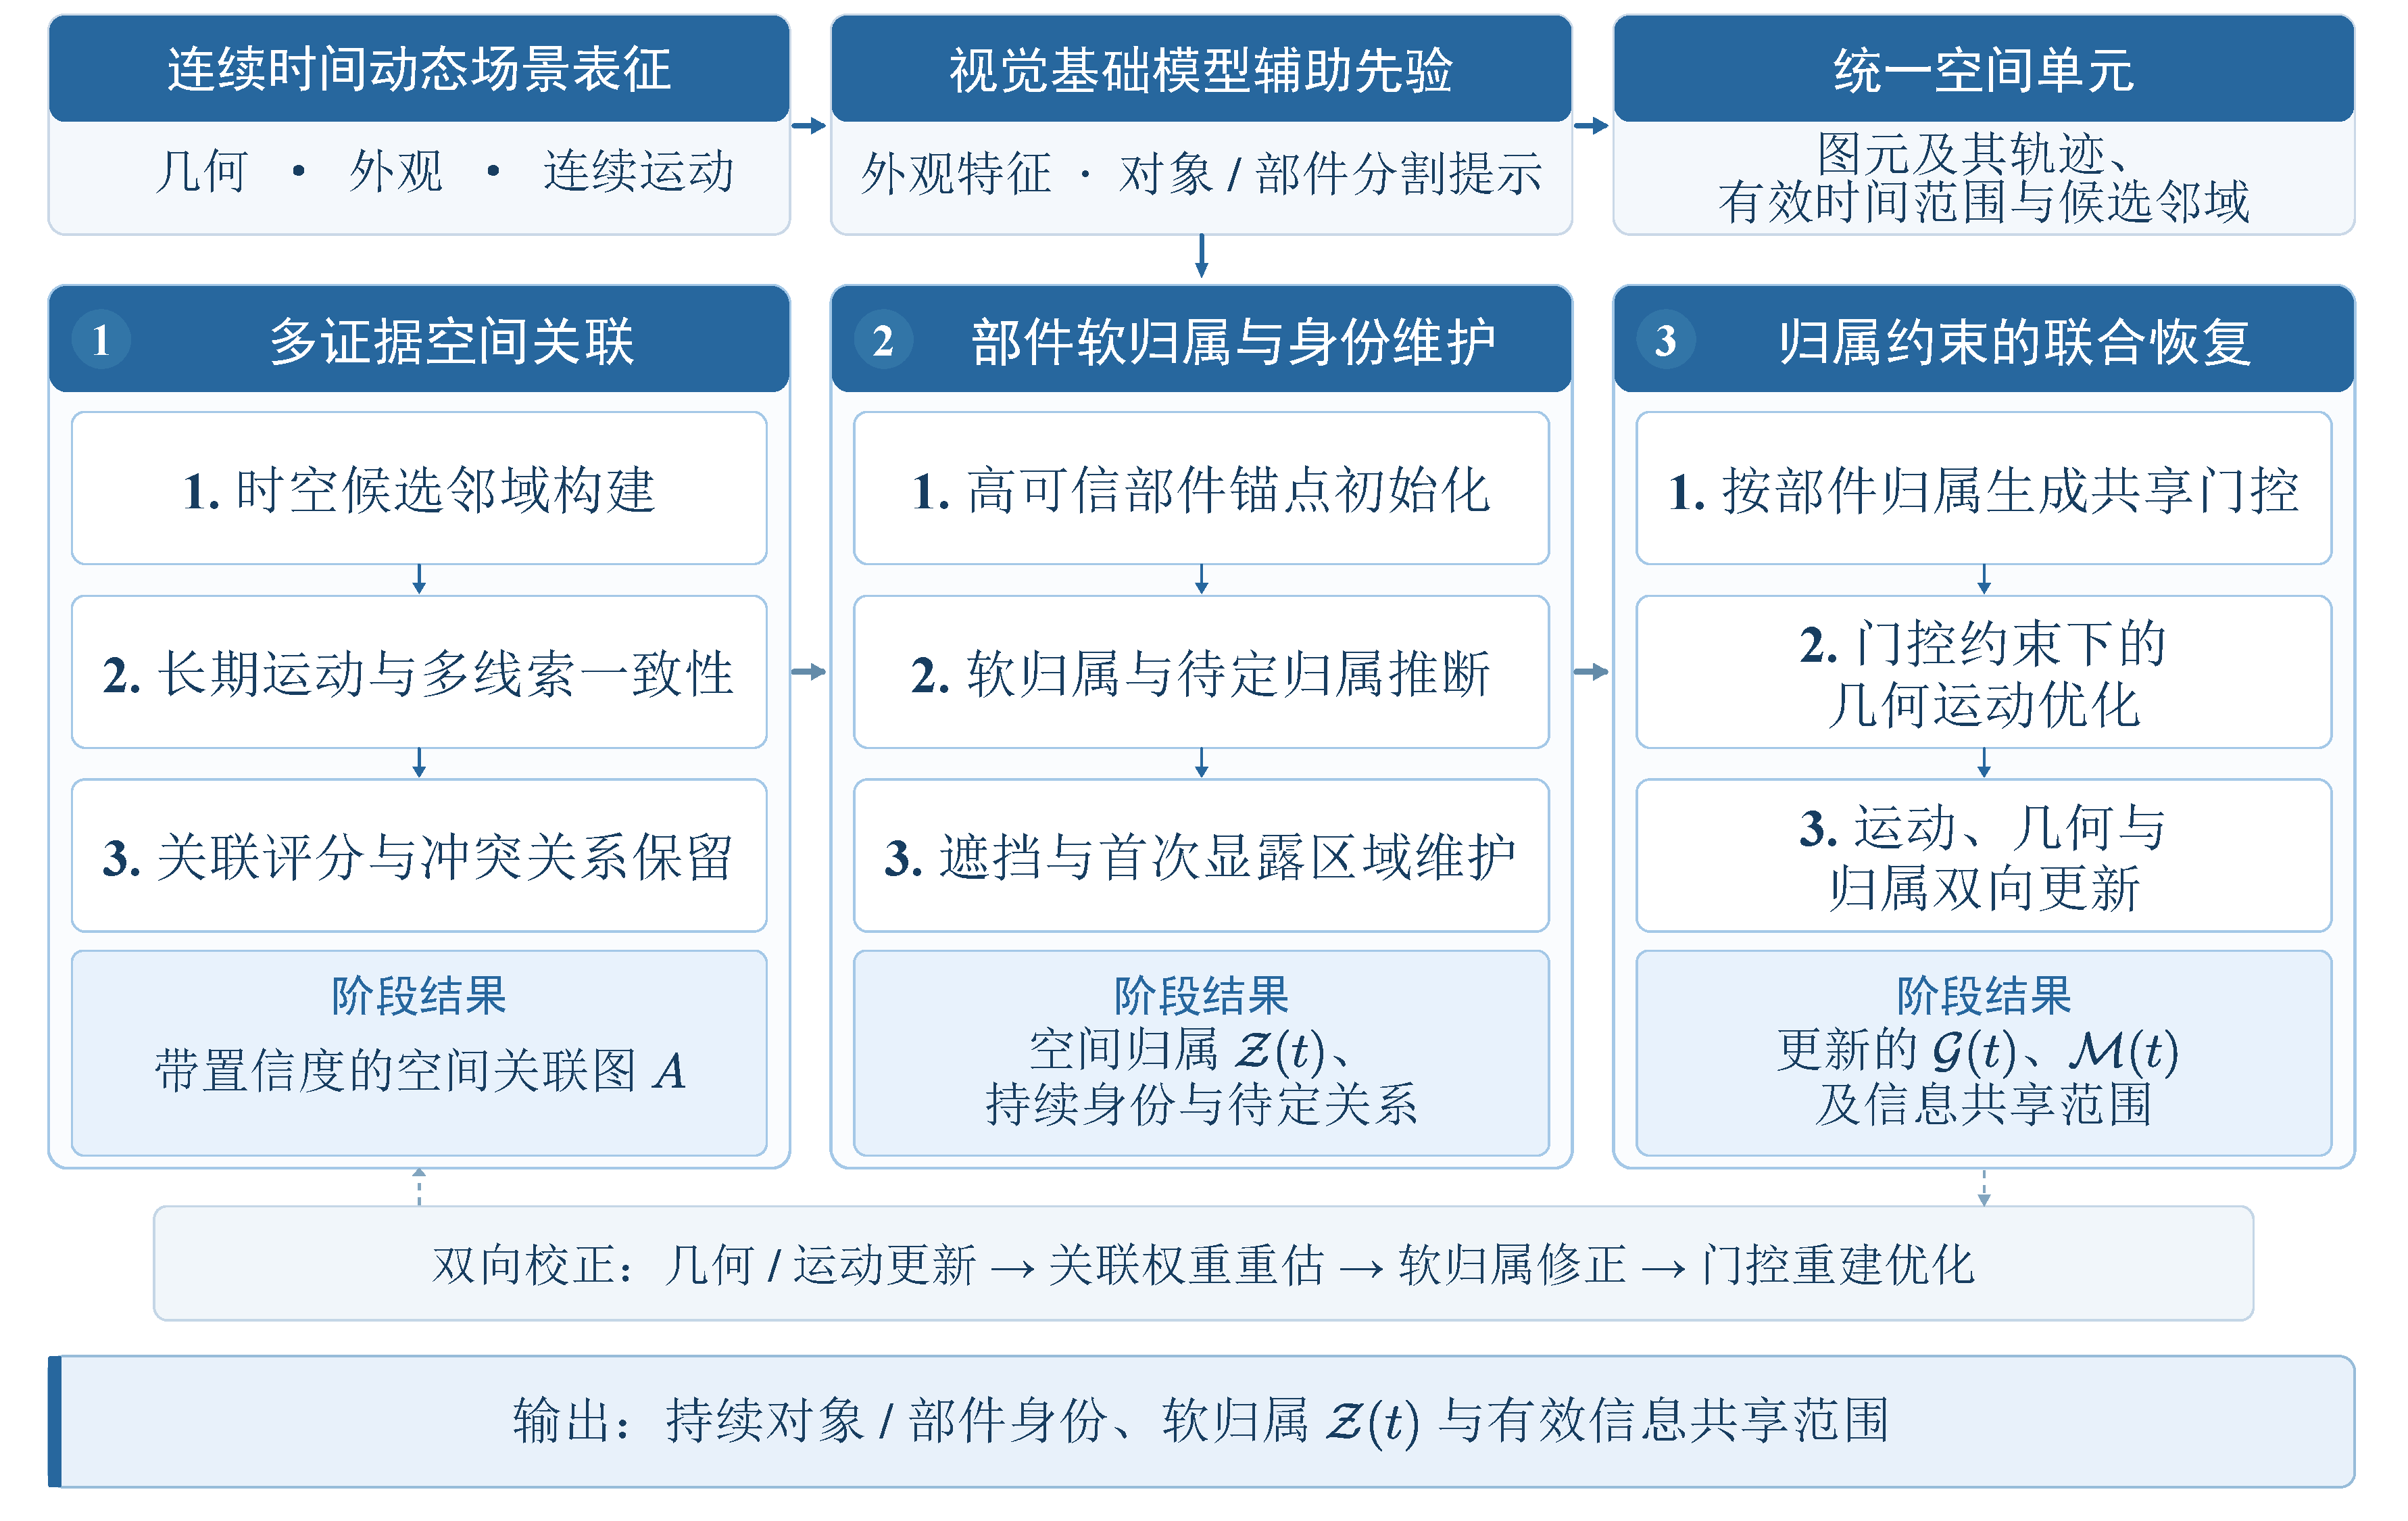
\includegraphics[width=\linewidth]{figures/chapters/ch03-plan/object-consistency-route/figure.pdf}
  \caption{连续运动引导的对象时空一致性建模技术路线}
  \label{fig:plan-route-object}
\end{figure}


\noindent\textbf{（1）多证据空间关联}

以第一项研究获得的几何 $\mathcal{G}(t)$、外观 $\mathcal{C}(t)$ 和连续运动 $\mathcal{M}(t)$ 为基础，将高斯图元及其运动轨迹组织为基本场景单元。首先根据空间邻近、轨迹覆盖及局部几何关系构建候选关联邻域，再结合长期相对运动、外观相似性和可见性信息，评价候选单元之间的空间关联。

考虑不同对象可能在部分时间区间内共同运动，而同一对象的不同部件也可能存在相对运动，拟利用较长时间范围内的运动变化及多线索一致性判断关联关系。设 $\Omega_{ij}(t)$ 为截至时刻 $t$ 用于分析场景单元 $i$ 和 $j$ 的有效观测窗口集合，分别累积支持共同部件归属与不同部件归属的证据：
\begin{equation}
  S_{ij}^{\pm}(t)
  =
  \sum_{\tau\in\Omega_{ij}(t)}
  \eta_{ij,\tau}e_{ij,\tau}^{\pm},
  \label{eq:route-object-evidence}
\end{equation}
其中，$e_{ij,\tau}^{+}$ 和 $e_{ij,\tau}^{-}$ 分别表示相应时间窗口内的正向关联与冲突证据，$\eta_{ij,\tau}$ 为结合轨迹可靠性、几何一致性及可见性确定的观测权重。通过多时刻证据积累，综合利用共同运动、相对运动变化和空间几何关系，提高关联判断的稳定性。

进一步考虑有效时间覆盖及不同关联解释之间的证据差异，构建关联可靠性：
\begin{equation}
  r_{ij}(t)
  =
  \frac{h_{ij}(t)}
       {h_{ij}(t)+\tau_0}
  \frac{
    \left|S_{ij}^{+}(t)-S_{ij}^{-}(t)\right|
  }{
    S_{ij}^{+}(t)+S_{ij}^{-}(t)+\epsilon
  },
  \label{eq:route-object-reliability}
\end{equation}
其中，$h_{ij}(t)$ 描述有效时间覆盖及运动变化提供的区分信息，$\tau_0$ 为调节参数，$\epsilon$ 为数值稳定项。利用 $r_{ij}(t)$ 对正向关联与冲突证据进行加权，建立带置信度的空间关联图 $\mathcal{H}(t)$，分别维护可信关联、冲突关系及待定关系。该关联图能够随新增观测持续更新，为对象及部件的空间组织提供多时刻证据。

\noindent\textbf{（2）部件软归属与身份维护}

在空间关联图的基础上，结合视觉基础模型提供的对象及部件分割先验，选择具有稳定跨时刻对应、较高观测覆盖和一致几何特征的场景单元作为身份锚点，并通过关联传播维护持续对象身份。考虑遮挡和局部形变引起的身份歧义，采用对象—部件层次化软归属表示，使对象级身份与部件级空间组织能够分别维护。

设当前存在 $K$ 个部件身份候选，对场景单元 $i$ 定义软归属向量：
\begin{equation}
  \mathbf{q}_i(t)=
  \left[
    q_{i,0}(t),
    q_{i,1}(t),\ldots,q_{i,K}(t)
  \right],
  \qquad
  \sum_{k=0}^{K}q_{i,k}(t)=1,
  \label{eq:route-object-soft-membership}
\end{equation}
其中，$q_{i,k}(t)$ 表示单元 $i$ 归属于部件 $k$ 的估计程度，$q_{i,0}(t)$ 表示当前归属待定。不同部件可通过层次关系关联到同一对象身份，从而同时描述对象身份的持续性与内部部件的相对运动。

综合身份锚点、空间关联与时序对应，建立软归属优化目标：

\begin{equation}
  \begin{aligned}
    \mathcal{L}_{\mathrm{attr}}
    ={}& \sum_{i\in\mathcal{S}} c_i\,\mathrm{CE}(\tilde z_i,\mathbf{q}_i)
    + \lambda_{+}\sum_{(i,j)\in\mathcal{A}^{+}}
    A_{ij}^{+}\|\mathbf{q}_i^{*}-\mathbf{q}_j^{*}\|_2^2\\
    &+ \lambda_{-}\sum_{(i,j)\in\mathcal{A}^{-}}
    A_{ij}^{-}\langle\mathbf{q}_i^{*},\mathbf{q}_j^{*}\rangle
    + \lambda_{\mathrm{temp}}\mathcal{L}_{\mathrm{temp}}
    + \lambda_{\mathrm{unk}}\mathcal{L}_{\mathrm{unk}}.
  \end{aligned}
  \label{eq:route-object-attribution-loss}
\end{equation}

其中，$\mathcal{S}$ 为可靠身份锚点集合，$\tilde z_i$ 和 $c_i$ 分别表示锚点身份先验及其可靠性，$\mathbf{q}_i^{*}$ 为已知部件的归属分量；$\mathcal{A}^{+}$、$\mathcal{A}^{-}$ 及其权重 $A_{ij}^{+}$、$A_{ij}^{-}$ 分别表示可信关联和冲突关系。$\mathcal{L}_{\mathrm{temp}}$ 用于保持可靠对应下的身份连续性，$\mathcal{L}_{\mathrm{unk}}$ 根据归属证据调节待定归属。通过正反关联约束与持续身份锚点相结合，提高遮挡和复杂运动条件下的空间归属一致性。

对于遮挡后重新出现的对象，利用持续身份、运动历史和外观特征恢复关联；对于首次显露的已有表面，结合当前几何与运动预测建立候选归属，并利用后续观测逐步完善空间组织。通过持续更新身份锚点和软归属关系，维护对象及部件的跨时刻一致性。

\noindent\textbf{（3）归属约束的联合恢复}

在建立对象及部件的空间归属后，进一步利用归属关系约束运动与几何信息的共享范围。考虑同一对象内部可能存在不同部件运动，而不同对象也可能短时共同运动，本项研究分别建立身份兼容与运动兼容约束，使运动信息的共享同时受到空间归属和局部运动一致性的控制。身份兼容用于判断几何单元与运动支撑是否属于相容的对象或部件，运动兼容则检验二者的共享能否解释局部轨迹及几何变化。对于同一对象内运动不同的部件，即使身份相容，仍依据运动证据限制跨部件共享；对于短时共同运动的不同对象，则通过身份约束避免仅凭运动相似而合并信息。两类证据共同决定共享强度，证据不足或相互冲突时降低共享权重并保留局部估计，从而在利用关联信息改善恢复的同时减少错误传播。

设几何单元 $i$ 与运动支撑节点 $j$ 的基础关联权重为 $\alpha_{ij}$，由部件软归属计算身份兼容程度 $g_{ij}^{\mathrm{id}}(t)=\sum_{k=1}^{K}q_{i,k}(t)q_{j,k}(t)$，并根据局部轨迹和几何运动残差估计运动兼容程度 $g_{ij}^{\mathrm{mot}}(t)$。综合两类约束，构建运动共享权重：
\begin{equation}
  \tilde{\alpha}_{ij}(t)
  =
  \frac{
    \alpha_{ij}
    g_{ij}^{\mathrm{id}}(t)
    g_{ij}^{\mathrm{mot}}(t)
  }{
    \displaystyle
    \sum_{\ell\in\mathcal{N}(i)}
    \alpha_{i\ell}
    g_{i\ell}^{\mathrm{id}}(t)
    g_{i\ell}^{\mathrm{mot}}(t)
  },
  \label{eq:route-object-sharing-weight}
\end{equation}
其中，$\mathcal{N}(i)$ 为候选运动支撑集合，$\alpha_{ij}$ 为局部运动关联。对归属与运动支持可靠的区域，按 $\tilde{\alpha}_{ij}(t)$ 更新图元变形；支持不足或归属待定时保留局部运动估计，以减少跨对象运动混合并表达部件相对运动。

将软归属约束并入第一项几何—运动恢复目标，联合优化模型为：
\begin{equation}
  \min_{\Theta_G,\Theta_C,\Theta_M,\Theta_Z}\quad
  \mathcal{L}_{\mathrm{joint}}
  = \mathcal{L}_{\mathrm{base}}
  (\Theta_G,\Theta_C,\Theta_M;\tilde{\alpha})
  + \lambda_{\mathrm{attr}}\mathcal{L}_{\mathrm{attr}},
  \label{eq:route-object-joint-objective}
\end{equation}
其中，$\mathcal{L}_{\mathrm{base}}$ 为几何—运动恢复目标，$\Theta_Z$ 为软归属参数，$\tilde{\alpha}$ 由归属及运动估计共同更新。优化时交替重估关联证据、更新软归属与共享权重，并联合恢复几何和运动，实现对象组织与动态表征的双向校正。

最终形成持续对象及部件身份、软归属 $\mathcal{Z}(t)$ 与有效共享范围，并同步完善几何 $\mathcal{G}(t)$ 和连续运动 $\mathcal{M}(t)$。拟在长期共动、部件相对运动、遮挡后重现及首次显露场景中，结合身份关联精度、运动恢复质量与机制消融，评估多时刻证据、软归属和共享约束的作用。



\subsubsection{结构约束关系变化下的动态场景表征维护}
\label{sec:plan-topology}

\begin{figure}[H]
  \centering
  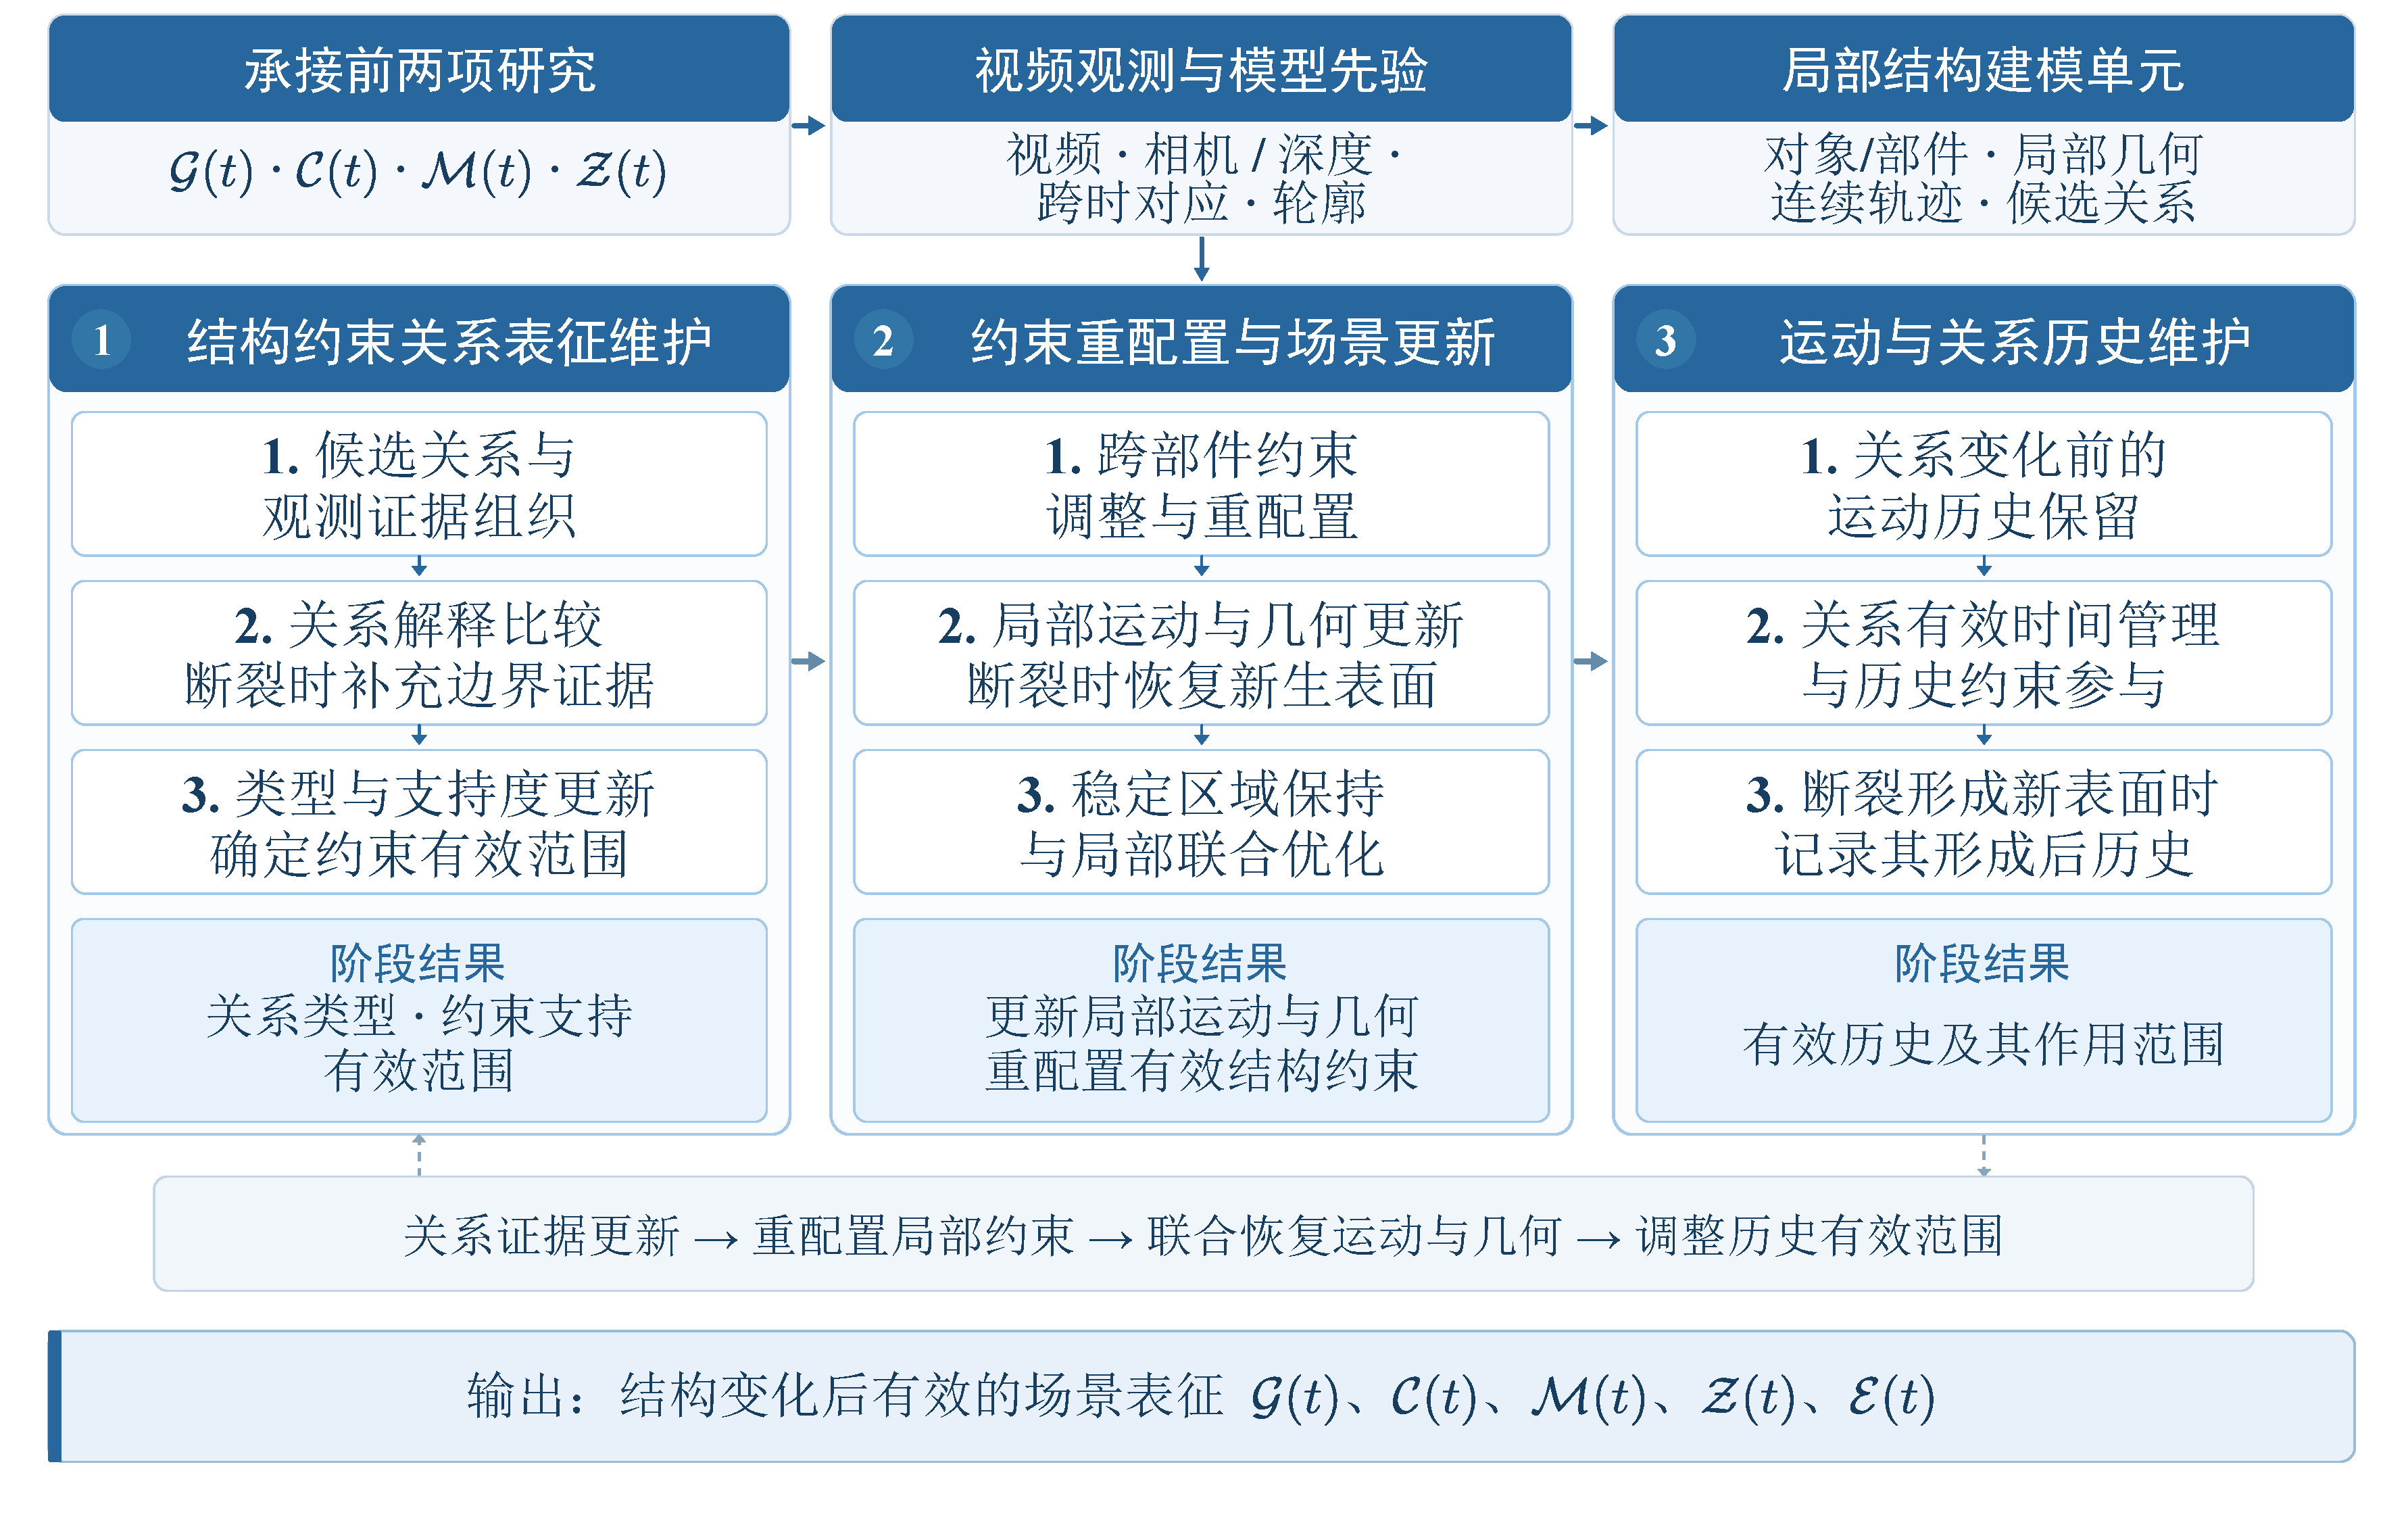
\includegraphics[width=\linewidth]{figures/chapters/ch03-plan/topology-change-route/figure.pdf}
  \caption{结构约束关系变化下的动态场景表征维护技术路线}
  \label{fig:plan-route-structure}
\end{figure}

本项研究面向部件装配关系或材料连续性改变引起的跨部件约束调整问题，拟研究结构约束关系表征维护、跨部件约束重配置与有效历史延续方法。关系有效时，利用跨部件观测共同约束运动与几何。关系改变后，调整或解除失效约束，分别维护相关区域的后续运动，并保留变化前仍有效的历史信息。具体技术路线如图~\ref{fig:plan-route-structure} 所示。



\noindent\textbf{（1）结构约束关系表征维护}

在已有连续动态场景表征的基础上，结合对象及部件的空间归属、局部几何与连续运动轨迹，构建候选结构约束关系集合 $\mathcal{E}_{\mathrm{cand}}$。空间邻近及短时共动提供候选关联线索，结构约束的成立需结合关系类型允许的相对运动与跨时刻观测一致性共同判断。对于候选关系 $e_{ij}$，综合上述证据及局部几何、可见性变化更新关系表征。

拟针对候选关系比较保持当前约束与调整其类型或作用范围两种关系解释，分别计算其对当前时序观测的解释误差，并综合跨部件运动不一致及适用时的边界变化证据构建如下关系调整评分
\begin{equation}
  \begin{aligned}
  D_{ij}(t)
  ={}&
  \mathcal{L}_{ij}^{\mathrm{keep}}(t)
  -\mathcal{L}_{ij}^{\mathrm{update}}(t)\\
  &-\lambda_{\mathrm{cmp}}\Delta\mathcal{C}_{ij}
  +\lambda_{\mathrm{sep}}S_{ij}(t)
  +\lambda_{\mathrm{bd}}B_{ij}(t),
  \end{aligned}
  \label{eq:route-structure-relation-score}
\end{equation}
其中，$\mathcal{L}_{ij}^{\mathrm{keep}}$ 和 $\mathcal{L}_{ij}^{\mathrm{update}}$ 分别表示保持当前关系约束、调整其类型或作用范围时的局部观测拟合误差，$\Delta\mathcal{C}_{ij}$ 表示关系调整所增加的模型复杂度，$S_{ij}(t)$ 描述观测运动与当前关系约束的不一致程度，$B_{ij}(t)$ 表示材料连续性改变时可用的新生边界证据。

进一步将关系调整评分映射为当前约束继续适用的支持程度
\begin{equation}
  p_{ij}^{\mathrm{rel}}(t)
  =
  \sigma\bigl(-\gamma D_{ij}(t)\bigr),
  \label{eq:route-structure-relation-support}
\end{equation}
其中，$p_{ij}^{\mathrm{rel}}(t)$ 表示当前关系约束继续适用的支持程度，$\gamma$ 为评分尺度参数。关系类型 $r_{ij}(t)$ 与支持程度共同构成关系表征。根据跨时刻观测调整关系类型、约束强度及有效范围，形成后续运动维护所需的关系信息。

\noindent\textbf{（2）跨部件约束重配置与场景表征更新}

在关系表征维护的基础上，将结构约束关系引入动态几何与运动优化。对于具有有效关系支持的区域，按关系类型所允许的相对运动和几何条件建立约束，其中装配关系可以对应受限的相对运动。关系改变时，根据更新后的类型与有效范围调整或解除跨部件约束，使后续运动能够分别维护。

设 $\ell_{ij}^{r_{ij}}(t)$ 表示候选关系 $e_{ij}$ 在关系类型 $r_{ij}$ 下的局部几何与运动约束误差，构建随关系支持程度变化的结构约束
\begin{equation}
  \mathcal{L}_{\mathrm{rel}}
  =
  \sum_{e_{ij}\in\mathcal{E}_{\mathrm{cand}}}
  \int_{\mathcal{T}}
    p_{ij}^{\mathrm{rel}}(t)
    \ell_{ij}^{r_{ij}}(t)\,\mathrm{d}t,
  \label{eq:route-structure-relation-loss}
\end{equation}
其中，$\mathcal{T}$ 为建模时间范围。$\ell_{ij}^{r_{ij}}$ 根据关系类型描述其允许的相对运动、几何连续性或局部形变。通过关系表征调节约束强度及作用范围，使各区域能够在关系有效时共同受观测约束，并在关系改变后分开维护后续运动。

关系改变后，根据新观测更新相关区域的几何和外观，并保持稳定区域的有效表征。材料断裂形成新表面时，初始化相应表面图元并恢复形成后的局部几何。遮挡解除后首次显露的已有表面按已有结构关联补充观测，共同完善几何和外观。

为协调局部结构更新与稳定区域已有表征的保持，构建如下局部联合优化目标
\begin{equation}
  \min_{\Theta_{\Omega}}\quad
  \mathcal{L}_{\mathrm{local}}
  = \mathcal{L}_{\mathrm{obs}}^{\Omega}
  + \lambda_{\mathrm{rel}}\mathcal{L}_{\mathrm{rel}}^{\Omega}
  + \lambda_{\mathrm{stable}}\mathcal{L}_{\mathrm{stable}},
  \label{eq:route-structure-local-objective}
\end{equation}
其中，$\Theta_{\Omega}$ 为结构约束关系变化影响区域及其邻域内待更新的几何、外观与运动参数，$\mathcal{L}_{\mathrm{obs}}^{\Omega}$ 综合局部图像、深度及轨迹观测约束，$\mathcal{L}_{\mathrm{rel}}^{\Omega}$ 为局部有效结构约束，$\mathcal{L}_{\mathrm{stable}}$ 用于保持稳定区域及边界邻域内已有几何与运动表征的一致性。

优化过程中，根据新增观测调整关系支持及约束范围，交替更新关系表征、局部运动参数和几何表征，并通过稳定区域约束延续已有信息。

\noindent\textbf{（3）运动历史、关系信息与表面历史维护}

拟通过局部运动历史、关系信息历史和适用时的表面形成历史，记录跨时刻观测已建立的场景信息，并依据关系约束的有效时间范围组织历史信息对后续表征构建的作用。相应的历史表示为
\begin{equation}
  \begin{aligned}
  \mathcal{H}(t)
  &=
  \left(
    \{\mathcal{T}_{i}^{\mathrm{mot}}\},
    \{\mathcal{Q}_{e}^{\mathrm{rel}}\},
    \{\mathcal{B}_{s}^{\mathrm{surf}}\}
  \right),\\
  \mathcal{T}_{i}^{\mathrm{mot}}
  &=
  \{(\tau,\mathbf{x}_{i}(\tau))\},\\
  \mathcal{Q}_{e}^{\mathrm{rel}}
  &=
  \{(\tau,r_e(\tau),p_e^{\mathrm{rel}}(\tau))\},\\
  \mathcal{B}_{s}^{\mathrm{surf}}
  &=
  \bigl(
    t_{s}^{\mathrm{birth}},
    t_{s}^{\mathrm{end}},
    v_s(\tau)
  \bigr),
  \end{aligned}
  \label{eq:route-structure-information-history}
\end{equation}
其中，$\mathcal{T}_{i}^{\mathrm{mot}}$ 为区域 $i$ 的运动历史。$\mathcal{Q}_{e}^{\mathrm{rel}}$ 记录关系 $e$ 的类型 $r_e$ 及约束支持 $p_e^{\mathrm{rel}}$ 随时间的变化，用于确定关系约束的有效时间范围。对于材料断裂形成的表面区域 $s$，$\mathcal{B}_{s}^{\mathrm{surf}}$ 记录其形成时刻 $t_{s}^{\mathrm{birth}}$、终止时刻 $t_{s}^{\mathrm{end}}$ 及可见性 $v_s(\tau)$，描述表面存在区间与观测可用性。

关系改变前由跨部件观测共同建立的运动历史予以保留。跨时间区间的运动与几何约束依据所依赖关系的有效时段参与优化，关系改变后的区域按新的关系类型及作用范围维护后续运动。稳定区域延续已有运动与几何信息，新生表面的历史从其形成时刻开始记录。

通过关系表征更新、跨部件约束重配置与有效历史延续，持续维护几何 $\mathcal{G}(t)$、外观 $\mathcal{C}(t)$、连续运动 $\mathcal{M}(t)$、对象归属 $\mathcal{Z}(t)$ 和结构关系 $\mathcal{E}(t)$，形成与当前结构约束相协调的动态场景表征。

拟从 IMPACT\cite{impact2026} 中组件状态或纠错标注明确的短片段，以及 \mbox{REASSEMBLE}\cite{reassemble2025} 中拆解阶段清楚的片段起步，截取关系保持与解除前后的局部窗口，在相同观测与历史条件下比较持续沿用旧约束、局部重配置和整体重置三种设置。验证重点包括关系有效阶段的联合运动恢复、关系改变后的分部件运动误差、稳定区域历史保持及失效约束残留。组件状态按已有标签粒度评价，运动与几何误差依据对应参考计算，关系表征与新生表面的直接评价限定于相应参考覆盖范围。结合变化部件与稳定区域的观测一致性检验表征维护效果，数据及标注条件见表~\ref{tab:data-sources}。




\subsubsection{动作后果预测与连续动态表征协同建模}
\label{sec:plan-response}

本项研究面向连续动态场景中的动作后果预测，采用“动态起点与动作条件编码—分类型关系与连续动力学—候选响应与预测反馈”的技术路线，如图~\ref{fig:plan-route-prediction} 所示。首先结合连续动态场景表征及交互历史，构建包含几何、运动、空间结构和响应相关信息的预测起点；随后利用分类型关系组织局部作用与响应传播，建立动作条件下的连续时间动力学模型；最后通过多步预测监督、候选响应推演及观测反馈，使连续动态表征与未来演化预测相互约束，形成可随交互过程持续更新的预测性世界模型。

\begin{figure}[H]
  \centering
  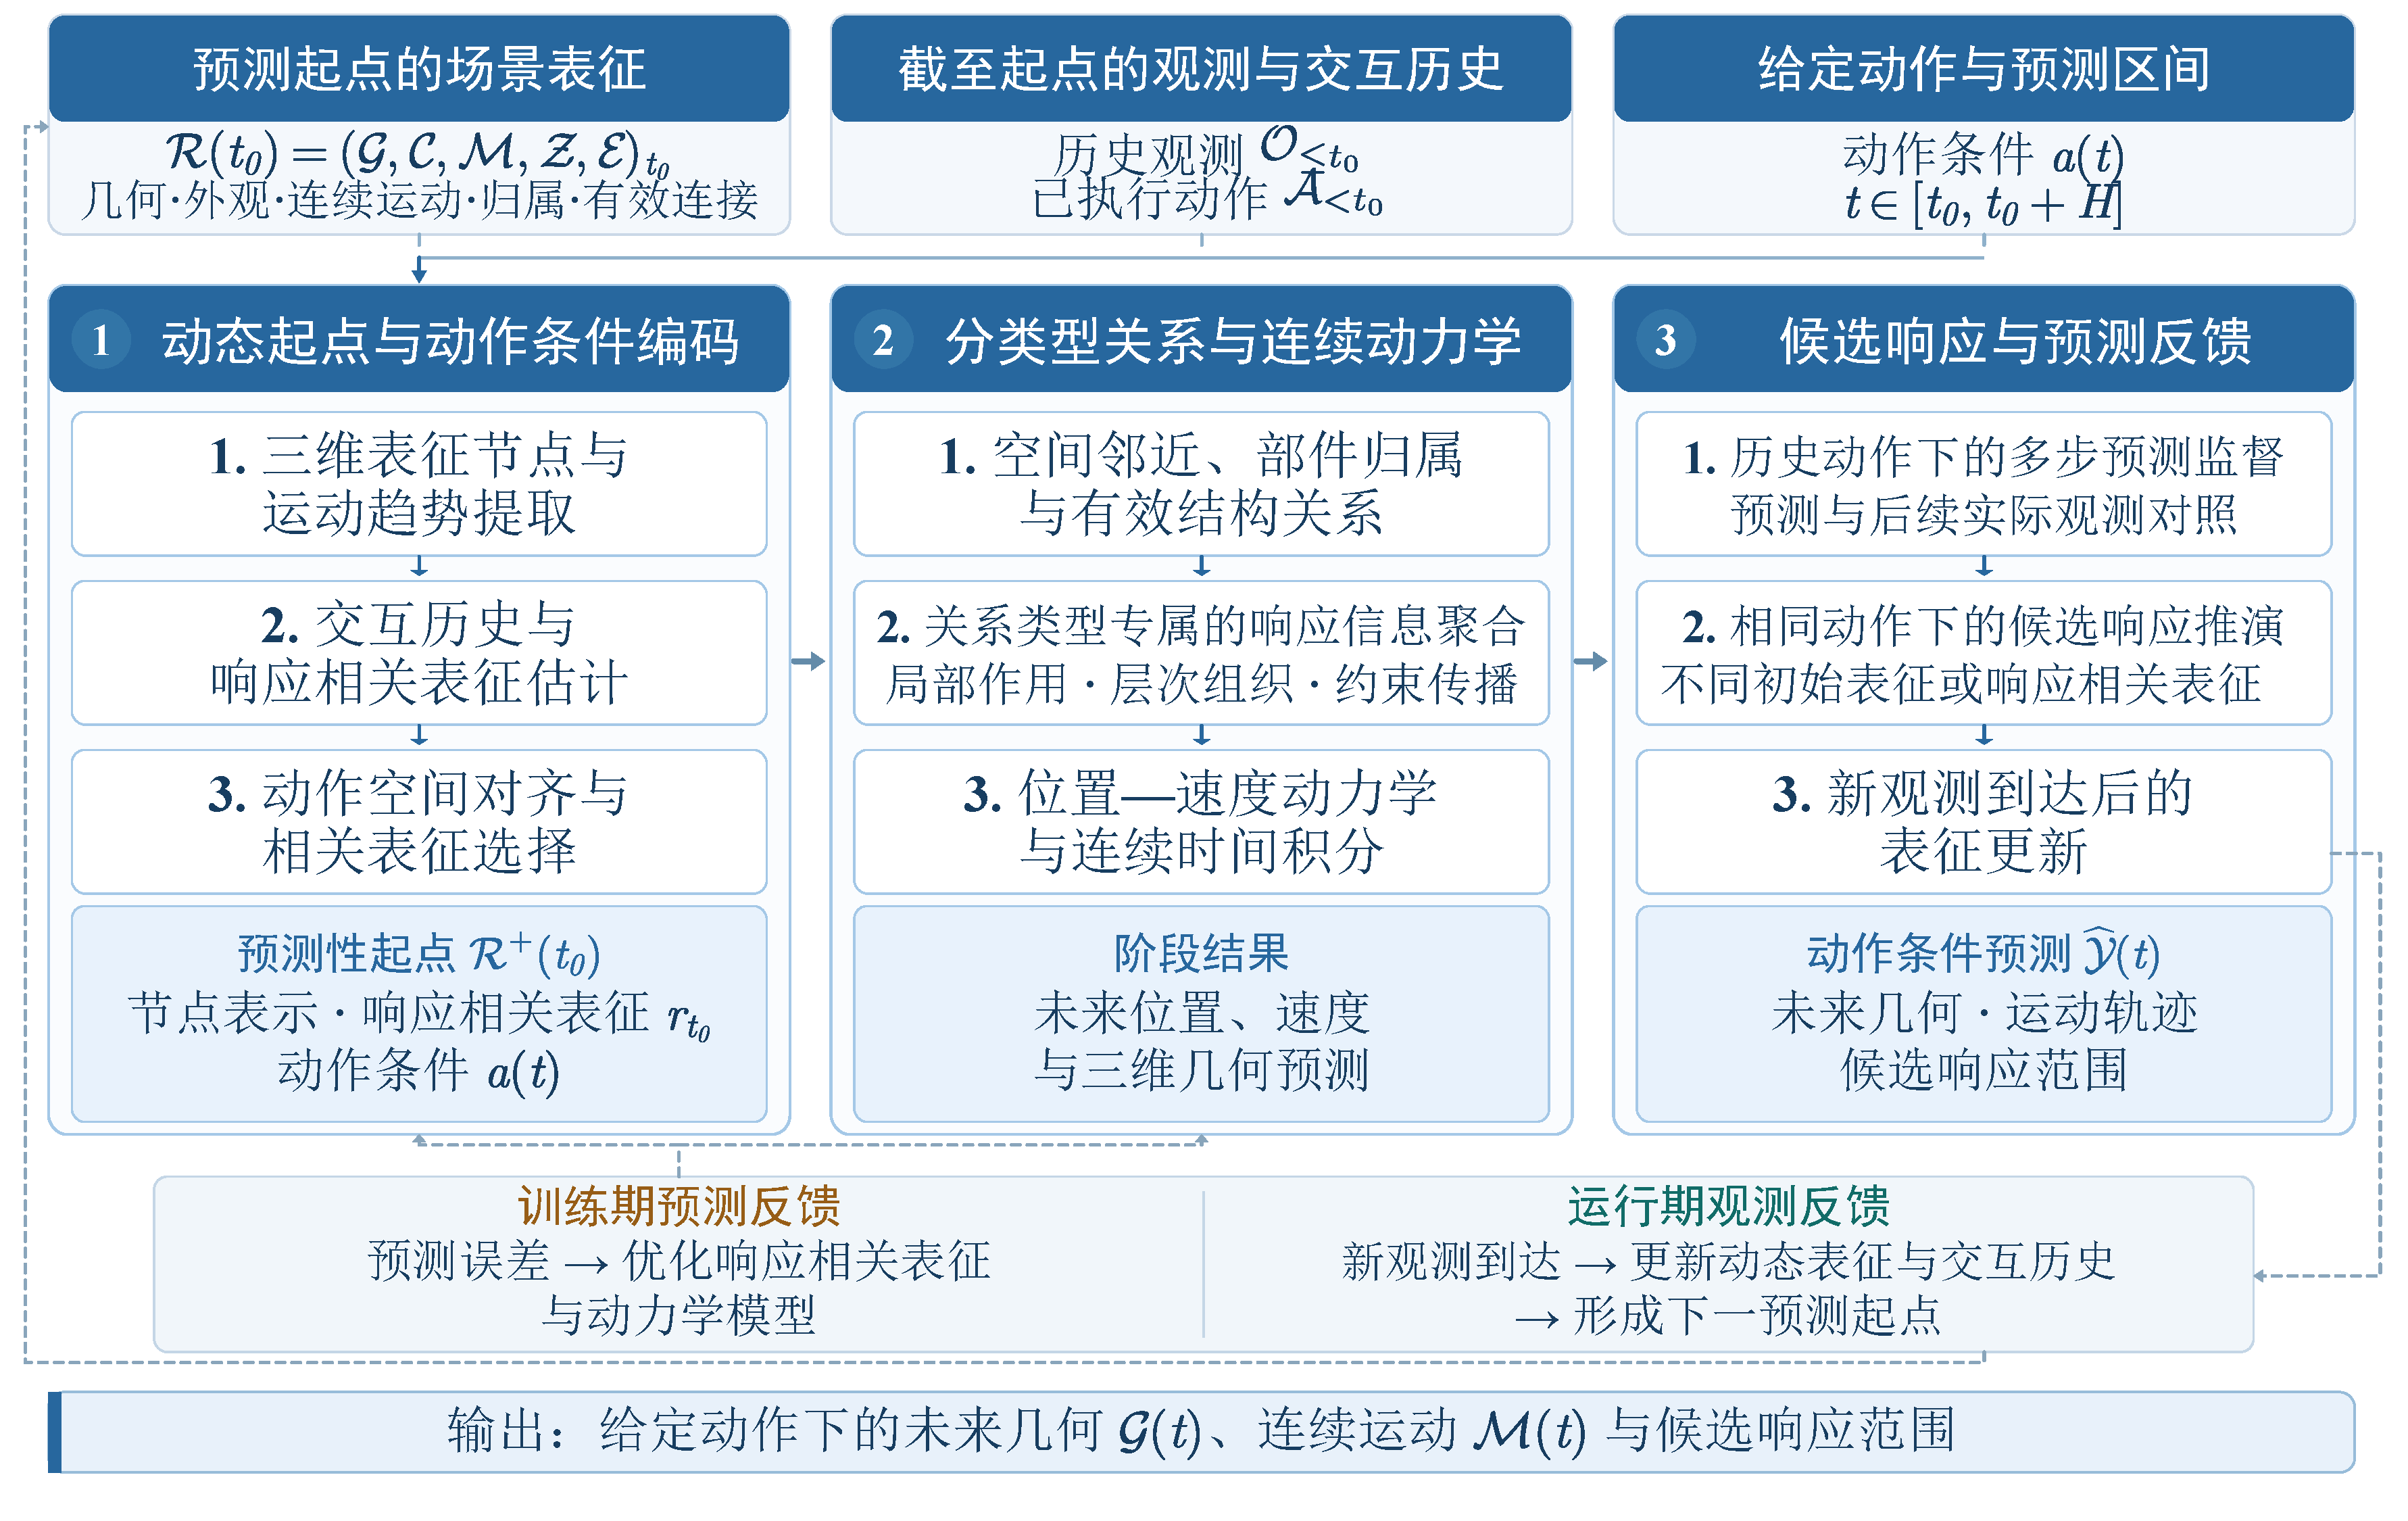
\includegraphics[width=\linewidth]{figures/chapters/ch03-plan/action-response-route/figure.pdf}
  \caption{动作后果预测与连续动态表征协同建模技术路线}
  \label{fig:plan-route-prediction}
\end{figure}


预测段内沿用起点时刻的有效结构约束关系，预测给定动作下的未来几何与运动响应。新观测到达后，更新动态场景表征，并从更新后的表征开始下一次预测。

\noindent\textbf{（1）动态起点与动作条件编码}

根据截至预测起点 $t_0$ 的可用观测构建连续动态场景表征 $\mathcal{R}(t_0)$，以其中的几何和运动信息组织三维表征节点。对于节点 $i$，构建包含三维位置 $\mathbf{x}_i(t_0)$、瞬时速度 $\mathbf{v}_i(t_0)$、局部几何与外观特征以及对象或部件归属的节点表征 $\mathbf{h}_i(t_0)$。其中，瞬时速度由连续时间运动表征求导获得，结构约束关系通过节点之间的关系类型及其当前有效范围表达。通过上述表征组织，将连续动态场景转换为适用于后续动力学预测的结构化初始条件。

考虑动作响应不仅受到当前几何与运动信息影响，还与已有交互过程中表现出的响应特性有关，拟结合截至预测起点的观测及已执行动作，学习响应相关潜在表征：
\begin{equation}
  r_{t_0}
  =
  F_{\phi}
  \left(
    \mathcal{R}(t_0),
    \mathcal{O}_{\leq t_0},
    \mathcal{A}_{<t_0}
  \right),
  \label{eq:route-response-latent-representation}
\end{equation}
其中，$\mathcal{O}_{\leq t_0}$ 和 $\mathcal{A}_{<t_0}$ 分别表示截至预测起点的观测历史与已执行动作历史，$F_{\phi}$ 为响应表征编码模型。潜在表征 $r_{t_0}$ 用于整合已有交互中反映的动力学及响应信息，与基础动态表征共同构成预测性世界表征 $\mathcal{R}^{+}(t_0)$。

对于给定的未来动作 $a(t)$，进一步根据动作类型、作用位置、持续时间及当前空间结构，将动作条件映射到相关三维表征节点。通过动作空间对齐与相关节点选择，构建节点级动作输入 $\mathbf{a}_i(t)$，使动力学模型能够区分直接受到动作作用的区域以及通过空间关系产生间接响应的区域。由此形成包含节点表征、响应相关潜在表征及动作条件的预测起点。

\noindent\textbf{（2）分类型关系与连续动力学}

在结构化预测起点的基础上，利用场景几何、对象归属及结构约束关系表征建立分类型空间关系。具体考虑空间邻近、对象或部件归属以及当前有效的结构约束三类关系，分别描述局部空间作用、层次化运动组织与跨部件约束。通过不同关系类型组织表征节点之间的信息传递，使动作影响能够沿相应的空间与结构关系传播。

设关系类型集合为 $\mathcal{Q}$，对于节点 $i$，构建类型专属的响应信息聚合：
\begin{equation}
  \mathbf{m}_i^{(r)}(t)
  =
  \sum_{j\in\mathcal{N}_r(i,t)}
  w_{ij}^{(r)}(t)
  \phi_r\left(
    \mathbf{h}_i(t),
    \mathbf{h}_j(t),
    \mathbf{x}_j(t)-\mathbf{x}_i(t)
  \right),
  \quad r\in\mathcal{Q},
  \label{eq:route-response-relation-message}
\end{equation}
其中，$\mathcal{N}_r(i,t)$ 为节点 $i$ 在关系类型 $r$ 下的关联邻域，$w_{ij}^{(r)}(t)$ 表示关系的有效程度，$\phi_r$ 为对应关系类型的消息函数。空间邻近关系根据预测过程中的几何位置更新，对象及部件关系提供层次化表征信息，结构约束关系则依据预测起点的关系类型和有效范围约束响应传播。通过关系类型专属的参数化与信息聚合，学习不同结构关系对局部运动和动作影响传播的作用。

进一步以节点的位置和速度作为主要动态变量，结合关系信息、响应潜在表征及动作条件，建立连续时间动力学模型：
\begin{equation}
  \begin{aligned}
  \frac{\mathrm{d}\mathbf{x}_i(t)}{\mathrm{d}t}
  &=
  \mathbf{v}_i(t),\\
  \frac{\mathrm{d}\mathbf{v}_i(t)}{\mathrm{d}t}
  &=
  f_{\theta}\left(
    \mathbf{h}_i(t),
    \{\mathbf{m}_i^{(r)}(t)\}_{r\in\mathcal{Q}},
    \mathbf{a}_i(t),
    r_{t_0}
  \right),
  \end{aligned}
  \label{eq:route-response-continuous-dynamics}
\end{equation}
其中，$f_{\theta}$ 为动作条件动力学模型，预测当前节点在节点表征、空间关系及外部动作作用下的速度变化率。通过连续时间数值积分获得未来节点的位置与速度轨迹，再利用节点运动驱动对应三维几何单元，恢复未来场景的动态几何与连续运动表征。

该模型将已有运动趋势作为动态初始条件，并通过分类型关系描述不同区域之间的响应传递，使未来运动预测同时受到几何、空间组织、当前有效的结构约束及交互历史的约束。通过对不同关系类型及表征信息的联合建模，研究连续动态表征对动作后果预测的作用。

\noindent\textbf{（3）候选响应与预测反馈}

利用包含动作记录和后续观测的交互序列开展多步预测训练。对于每个预测起点 $t_0$，表征重建、初始化与候选筛选均使用截至 $t_0$ 的观测和已执行动作历史。给定后续动作序列，模型递推预测未来三维位置、运动轨迹及几何变化。$t_0$ 之后的观测在训练阶段用于计算多步预测监督，在验证和测试阶段用于评价预测结果。

考虑有限观测可能对应不同的初始运动估计和响应相关潜在表征，进一步构建多组候选预测起点，在相同动作条件下分别进行连续动力学推演：
\begin{equation}
  \widehat{\mathcal{Y}}_{t_0:t_0+H}^{(s)}
  =
  \operatorname{Rollout}_{\theta}
  \left(
    \mathbf{H}_{t_0}^{(s)},
    r_{t_0}^{(s)},
    a_{t_0:t_0+H}
  \right),
  \label{eq:route-response-candidate-rollout}
\end{equation}
其中，$\mathbf{H}_{t_0}^{(s)}$ 和 $r_{t_0}^{(s)}$ 分别表示第 $s$ 组候选节点表征与响应潜在表征，$a_{t_0:t_0+H}$ 为给定动作序列，$\operatorname{Rollout}_{\theta}$ 表示连续动力学积分与几何恢复过程。通过比较不同候选起点在相同动作下的演化结果，获得未来几何、运动轨迹及候选响应范围，并分析初始表征差异对预测结果的影响。

为使动态表征与动作预测相互促进，拟将多步预测监督与已有观测下的表征一致性约束相结合，构建协同优化目标：
\begin{equation}
  \min_{\theta,\phi,\Theta_R}\quad
  \mathcal{L}_{\mathrm{joint}}
  = \lambda_{\mathrm{traj}}\mathcal{L}_{\mathrm{traj}}
  + \lambda_{\mathrm{render}}\mathcal{L}_{\mathrm{render}}
  + \lambda_{\mathrm{hist}}\mathcal{L}_{\mathrm{hist}}
  + \lambda_{\mathrm{reg}}\mathcal{L}_{\mathrm{reg}},
  \label{eq:route-response-joint-objective}
\end{equation}
其中，$\theta$ 和 $\phi$ 分别为动力学模型与响应表征编码模型的参数，$\Theta_R$ 表示参与协同优化的动态表征参数。$\mathcal{L}_{\mathrm{traj}}$ 约束多步预测轨迹，$\mathcal{L}_{\mathrm{render}}$ 利用未来图像及可用深度观测约束预测几何，$\mathcal{L}_{\mathrm{hist}}$ 保持已有观测下的几何与运动表征一致性，$\mathcal{L}_{\mathrm{reg}}$ 为动力学及响应潜在表征的正则约束。对于具有可靠三维轨迹参考的序列，引入三维运动监督；对于主要提供视觉观测的序列，则利用投影轨迹与可微渲染建立预测约束。

优化采用分阶段训练与联合调整相结合的方式：首先基于已有连续动态表征训练响应表征编码与动作条件动力学模型，建立稳定的未来演化预测；随后利用多步预测误差联合优化响应相关潜在表征及可训练的动态表征参数，使内部表征进一步保留影响动作响应的信息，同时维持已有观测下的几何与运动一致性。

在连续交互过程中，模型保存当前预测结果。新观测及动作执行反馈到达后，更新连续动态场景表征与交互历史，并估计新的响应相关潜在表征，形成下一预测起点。通过预测监督与观测更新两个过程，建立动态场景表征维护、动作条件演化预测及实际反馈相联系的时序闭环。

最终形成给定动作条件下的未来几何 $\widehat{\mathcal{G}}(t)$、连续运动 $\widehat{\mathcal{M}}(t)$ 及候选响应范围。拟通过多步三维轨迹预测、未来几何重建及不同动作条件下的比较，结合表征分量消融与估计误差扰动，分析连续运动、对象归属、结构约束关系和响应潜在表征对预测结果的作用，验证动态表征与动作条件预测协同建模的有效性。起步可从 DROID\cite{droid2024} 中筛选动作记录明确、主要运动区域可跟踪的短片段，以动作前历史构建预测起点，仅输入记录的后续动作，先评价短时轨迹与几何预测，再逐步延长预测时域；利用 PointWorld-DROID\cite{ref06} 的三维点流及有效性标记评价可跟踪区域，并在固定历史、动作及响应模型的条件下比较连续运动、对象归属和结构约束信息的作用。由于该点流为自动估计结果，应作为带不确定性的参考而非无误差真值；缺少直接轨迹参考时，结合可用观测进行投影轨迹或渲染几何一致性评价。PhysTwin\cite{phystwin2025} 的少量手工轨迹点可在与动作历史能够对齐的片段中补充轨迹评价，并按其参考范围解释结果。


\npuTemplateHeading{2.研究计划可行性，研究条件落实情况，可能存在的问题及解决办法（可续页）}
\subsection{研究计划可行性分析}

本课题以已有动态场景建模和动作条件表征学习为基础，分阶段推进连续时间表征、空间结构、结构关系变化和动作响应四项研究。四项研究围绕同一连续动态场景表征展开，分别形成运动与几何恢复、对象空间组织、关系更新及动作条件预测的方法，并通过明确的输入、输出和评价目标保持研究边界清晰。

\textbf{理论与方法依据。}连续时间运动、跨时空关联、动态表面建模和动作条件演化均已有可借鉴的理论与方法。现有时序视觉、三维表示和状态空间建模方法，为各阶段的表征构建、状态更新及未来演化预测提供了方法基础。研究将依据各项任务的观测条件和目标选择相应的表示与评价方式，逐项实现，并通过基线比较、控制变量和模块消融检验关键机制；在单项方法具备稳定结果后，再研究模块间的信息传递及联合效果。

\textbf{前期工作积累。}CoFuse4D 为带噪对应融合、稀疏运动支撑及连续时间建模提供了实现经验，相关实验初步验证了融合跨时刻对应并组织动态运动的可行性；PS-VLA 建立了动作条件状态转移、观测更新与执行反馈相结合的建模流程，为持续维护预测状态提供研究基础。两项工作尚未发表，仅作为研究起点；对象空间归属、结构约束关系变化后的表征维护，以及这些信息对动作预测的作用仍需在本课题中研究和验证。

\textbf{实施与验证路径。}四项研究先依托已有表示和公开数据独立验证，再通过共同表征接口逐步衔接。实验从观测与参考较明确的条件起步，逐步增加场景变化和交互因素；在评价某一环节时，固定其他模块或采用简化设置，以区分各组成部分的作用。对于相互衔接的环节，再开展逐步增加模块的对比实验，检查表征传递、预测效果和误差变化。该安排使各项研究均可形成独立阶段成果，并为后续联合验证提供基础。

\subsection{研究条件落实情况}

本课题依托陕西省信息获取与处理重点实验室开展，现有计算平台、软件基础、机器人设备及公开数据可支撑算法开发与比较实验。研究条件覆盖离线建模、模型训练、数据集评价和操作条件下的实机验证，可按研究阶段组织使用。

\textbf{计算与软件条件：}实验室配备 16 张 \mbox{NVIDIA RTX PRO 6000D} GPU，单卡显存 84\,GB，可支持动态数据处理、模型训练及并行对比实验。已有数据处理、三维建模和评测工具可用于建立实验流程；研究中将按模型规模安排资源，并记录软件依赖、数据划分和主要实验设置，以支持结果复核。

\textbf{机器人实验条件：}实验室现有两台机械臂，可为动作执行和操作条件下的实机验证提供设备基础。拟根据方法成熟度分阶段安排验证，先在可控条件下检查动作执行、状态观测与预测结果，再逐步开展实机实验；通过统一操作流程、记录实验条件并重复必要试验，支持结果比较和稳定性分析。

\textbf{数据与验证条件：}现有公开数据涵盖动态场景、多视角观测、轨迹标注及机器人交互等类型，主要数据规模、观测和标注见表~\ref{tab:data-sources}。各项研究可依据可用数据开展相应的模型训练、定量比较和机制分析，并结合机械臂实机条件补充操作过程中的验证。

\begin{table}[H]
  \centering
  \caption{公开数据源及主要数据属性}
  \label{tab:data-sources}
  {
  \renewcommand{\arraystretch}{1.12}
  \setlength{\tabcolsep}{2.2pt}
  \renewcommand{\tabularxcolumn}[1]{>{\raggedright\arraybackslash}m{#1}}
  \begin{tabularx}{\linewidth}{@{}>{\raggedright\arraybackslash}m{38mm}>{\raggedright\arraybackslash}m{18mm}>{\raggedright\arraybackslash}m{39mm}X@{}}
    \hline
    \textbf{数据集} & \textbf{类型} & \textbf{数据规模} & \textbf{主要观测与标注} \\
    \hline
    \textbf{DyCheck iPhone}\cite{dycheck2022} & 真实 & 14 段；28 GB & 单目 RGB、相机、深度与关键点 \\
    \textbf{PointOdyssey}\cite{pointodyssey2023} & 合成 & 159 段；2,000 帧/段 & RGB-D、实例与 2D/3D 轨迹 \\
    \textbf{Nerfies}\cite{nerfies2021,hypernerf2021} & 真实 & 7 段 & 动态多视角视频 \\
    \textbf{Syn4D}\cite{syn4d2026} & 合成 & 4,700 段；140 万帧 & 多视角 RGB、深度与稠密轨迹 \\
    \textbf{Deform360}\cite{deform3602026} & 真实 & 198 对象；1,980 段；215.7 h & 多视角视频、触觉、3D 粒子轨迹 \\
    \textbf{DROID}\cite{droid2024} & 真实 & 7.6 万示范；350 h & 多视角视频、动作记录 \\
    \textbf{PointWorld-DROID}\cite{ref06} & 派生 & 多 TB & 三维点流与有效性标记 \\
    \textbf{PhysTwin}\cite{phystwin2025} & 真实 & 22 场景；每段 1--10 s & RGB-D 视频与手工轨迹点 \\
    \textbf{IMPACT}\cite{impact2026} & 真实 & 112 试验；13 人；39.5 h & 多视角 RGB-D、组件状态、纠错标注 \\
    \textbf{REASSEMBLE}\cite{reassemble2025} & 真实 & 4,551 示范；17 对象；781 min & 多视角 RGB、事件、力/力矩、音频 \\
    \hline
  \end{tabularx}}
\end{table}

各项实验可依托现有数据处理、建模与评测工具分阶段开展，先完成分项方法的开发和验证，再逐步组织协同实验。代码版本、运行环境、数据划分及主要实验设置统一记录，便于结果复核与后续比较。

\subsection{可能存在的问题及解决办法}

研究实施可能受到数据条件、计算资源及实机实验组织等因素影响，拟结合阶段目标安排研究任务与验证方式。

\begin{enumerate}[label=（\arabic*）,leftmargin=2.4em,labelsep=0.3em,
    itemsep=0.8ex,topsep=0.4ex,parsep=0pt]
    \item \textbf{数据条件与验证安排。}
    不同研究环节所需的观测类型与数据规模有所差异，数据条件可能影响实验安排和验证覆盖。拟结合阶段目标统筹选择可用数据，合理安排处理与验证工作，并根据阶段进展完善实验方案。

    \item \textbf{计算资源与实验周期。}
    模型训练和动态数据处理需要一定计算资源，实验周期也可能随任务进展变化。拟根据阶段目标和模型规模安排计算资源，优先完成关键方法与必要验证，并结合实际进展调整实验规模和时间安排。

    \item \textbf{机械臂实机验证与变量控制。}
    实机实验涉及设备运行、动作执行和实验条件协调，重复验证及变量控制需要较细致的安排。拟逐步完善实验流程，统一主要操作条件并记录实验过程，结合重复实验检验结果稳定性；先通过可控实验开展方法验证，再逐步进行机械臂实机验证。
\end{enumerate}

\newpage
\npuTemplateHeading{3.研究计划及预期成果}
\npuSchedule{%
  \textbf{2026.10--2027.03} & 完成开题及相关文献梳理，完善 CoFuse4D 和 PS-VLA 前期工作并按进展投稿；建立实验基础，研究观测置信度约束的连续运动恢复，开展初步比较。形成开题报告、实验基线和阶段论文稿件。 \\[3pt]\hline
  \textbf{2027.04--2027.09} & 完善不确定性感知的连续时间场景表征，分析采样和观测质量的影响；研究连续运动引导的空间归属与结构组织，开展多场景比较和关键消融。形成方法实现、实验分析及阶段研究稿件。 \\[3pt]\hline
  \textbf{2027.10--2028.03} & 研究结构约束关系变化后的运动维护与局部更新，开展公开序列上的比较及历史保持、约束重配置消融；并行开展动态初始条件下的动作后果预测建模。形成结构关系适应和动作预测的阶段方法及实验结果。 \\[3pt]\hline
  \textbf{2028.04--2028.10} & 完善公开交互数据上的动作响应预测验证，开展模型衔接、误差传递和失败情形分析；整理研究成果，完成博士学位论文撰写与修改，按学校安排推进送审及答辩。形成研究原型、可复核验证协议及论文。 \\
}

\subsection{预期创新点及成果形式}

本课题预期形成连续动态世界模型构建方法及研究原型，积累可复核的比较、消融与误差分析结果，形成学术论文和博士学位论文。拟取得的创新性认识与方法进展如下，其有效性和成立范围通过上述验证确定。

（1）\textbf{观测支持与时间表达能力的联合配置机制。}将观测置信度、有效时间覆盖及局部运动自由度纳入同一求解过程，研究证据强弱与表达能力的匹配关系，形成兼顾非采样时刻恢复和快速运动保持的连续时间表征方法。

（2）\textbf{连续运动与空间归属的双向约束机制。}以持续相对运动联合几何、外观和可见性推断软归属，再由归属限定共享约束，形成运动、几何与空间组织相互校正的方法，阐明遮挡和短时共动下信息共享的有效条件。

（3）\textbf{结构约束关系变化下运动维护与历史延续的协调机制。}关系有效时利用跨部件观测共同约束运动，关系改变后按新的有效范围维护各区域运动，并保留仍有效的历史；材料断裂及新生表面作为其中一种情形，形成面向结构约束关系变化的连续动态场景表征维护方法。

（4）\textbf{运动与当前结构约束的动作响应建模机制。}从相同历史构建动态初始信息，通过分类型关系组织响应并传播关键解释分歧，研究运动、归属和连接对预测的作用及误差传递，明确连续动态表征的有效条件与可替代范围。
